 \documentclass[11pt,a4paper]{report}
%%% Preamble %%%

% Packages: I comment ones I don't need or am not using to cut down on compiling time.

	% Default: AMS maths packages

		\usepackage{amsmath}
		\usepackage{amssymb}
		\usepackage{amsfonts}
		\usepackage{mathtools}
	%	\mathtoolsset{showonlyrefs}

	%		\usepackage[amsmath,thmmarks]{ntheorem}

	% Geometry: The layout of the document.

		\usepackage[margin=1.4in]{geometry}

	%  	\usepackage[width = 15 cm, left = 3 cm, height = 23 cm, top = 3 cm]{geometry} % A4 Paper, W = 21 cm, H = 29.7 cm. Paperwidth = left + w`'idth + right, Paperlength = top + height + bottom.

	 	\usepackage{multicol} % Used to switch to two column mode.
	 	\setlength{\columnsep}{0.75cm} % Determines the length between columns

	% Graphics: Allows images.

	 	\usepackage{graphicx} % Used to include images.
	% 	\usepackage{epstopdf} % Required in pdflatex for eps images.
	 	\usepackage{float} % For figures in multicolumn`'
	% 	\usepackage{wrapfig} % Used to have multiple figures in a single beamer slide.

	% 	\graphicspath{ {./Figures/} } % The location of figures used in this document.

	% Diagrams: Diagram creation.

	 	\usepackage{tikz} % Creates diagrams, needs calc for arithmatic.
		\usepackage{tikzscale}
	 	\usepackage{pgfplots}
	 	\usepackage{calc}

	% Figures: Extends figure functionality, allows multiple figures per float environment.

	 	\usepackage{caption} % Needed for subcaption.
	 	\usepackage{subcaption} % Allows creation of subfigures, which allows multiple labelled figures per environment.
	 	\usepackage{tabu}

	 	\pgfplotsset{compat=1.12}

	% Tables: Extends table functionalirt, allows multiple page tables.

	 	%\usepackage{xtab} % Extended tables.

	% Titles: Modifies titles, especially for multicolumns

	% 	\usepackage{titlesec}

	% 	\titleformat{\section}
	% 		{\normalfont\Large\bfseries\centering}
	% 		{\thesection}{1ex}{}

	% 	\titleformat{\subsection}
	% 		{\normalfont\large\bfseries\centering}
	% 		{\thesubsection}{1ex}{}

	% Theorems: Defines theorems, axioms, definitions, etc in a custom environment.

	% 	\usepackage{amsthm} % Needed for the definitions

	% 	%This style is in italics and can be used as a subsection
	% 	\newtheoremstyle{conditionStyle}% Name
	% 		{3pt}% Space above
	% 		{3pt}% Space below
	% 		{}% Body font
	% 		{\parindent}% Indent amount
	% 		{\itshape}% Theorem ead font
	% 		{:}% Punctuation after theorem ead
	% 		{.5em}% Space after theorem ead
	% 		{}% Theorem head spec (can be left empty, meaning `normal')

	% 	\newtheoremstyle{solutionStyle}% name of the style to be used
	% 		{3pt}% measure of space to leave above the theorem. E.g.: 3pt
	% 		{3pt}% measure of space to leave below the theorem. E.g.: 3pt
	% 		{}% name of font to use in the body of the theorem
	% 		{}% measure of space to indent
	% 		{\bfseries}% name of head font
	% 		{:}% punctuation between head and body
	% 		{.5em}% space after theorem head; " " = normal interword space
	% 		{}% Manually specify head

	% 	\newtheorem{axiom}{Axiom}
	% 	\newtheorem{property}{Property}
	% 	\newtheorem{rl}{Rule}
	% 	\newtheorem{law}{Law}		
	% 	\newtheorem{thm}{Theorem}
	% 	\newtheorem{ex}{Example}
	% 	\newtheorem{prn}{Principle}
	% 	\newtheorem{prf}{Proof}

	% 	\theoremstyle{definition}
	% 	\newtheorem{exc}{Excercise}
	% 	\newtheorem{defn}{Definition}
	% 	\newtheorem{clm}{Claim}
	% 	\newtheorem{sol}{Solution}	
	% 	\newtheorem{qst}{Question}

	% 	\theoremstyle{conditionStyle}
	% 	\newtheorem{condition}{Condition}[rl]

	% 	\theoremstyle{solutionStyle}
	% 	\newtheorem{qsol}{Solution}[qst]

	% Utility: Packages that add extra functionality.

	% 	\usepackage{xcolor} % Used to make footnote numbering red.
	 	\usepackage{esdiff} %easy differentials eg. \diff[n]{y}{x}, \diffp[n]{y}{x}.
	 	\usepackage{verbatim} % Used to write code.
	% 	\usepackage{lipsum} % Generates Lorem Ipsum.
	%	\usepackage{textcomp} % Provides roman greek letters.
	% 	\usepackage{eurosym} % Provides accurate euro symbol.
	% 	\usepackage{enumerate} % Needed for lists that use lower case roman numerals.

	% Datetime: Changes the date.

		\usepackage[UKenglish]{isodate}% Used to change the date format.
		\cleanlookdateon % Removes the ordinal suffix

	% Siunitx: has a good implimentation for using units within latex
		\usepackage{siunitx}
		% example command is \SI{}{\micro\meter}

	% Makes the pages look more fancy

		\usepackage{fancyhdr}
		\pagestyle{fancy}

		\fancyhf{}
		\fancyhead[LE]{\rightmark}
		\fancyhead[RO]{\leftmark}
		\fancyfoot[C]{\thepage}

		\setlength{\headheight}{15.0pt}
		\renewcommand{\footrulewidth}{0.4pt}

		% Page Style of new chapter pages.
		\fancypagestyle{plain}{%
			\fancyhf{} % clear all header and footer fields
			\fancyfoot[C]{\thepage} % except the center
			\renewcommand{\headrulewidth}{0pt}
			\renewcommand{\footrulewidth}{0.4pt}
		}

	% Custom accents

	% \usepackage{accents}
	
	% \newlength{\dtildeheight}
	% \newcommand{\doubletilde}[1]{%
	%     \settoheight{\dtildeheight}{\ensuremath{\tilde{#1}}}%
	%     \addtolength{\dtildeheight}{-0.35ex}%
	%     \tilde{\vphantom{\rule{1pt}{\dtildeheight}}%
	%     \smash{\tilde{#1}}}}

	% Tocbibind: These settings put the bibliography into the contents
		%\usepackage[nottoc]{tocbibind}

	% BibLaTeX: The citestyles and bib file used in citations are edited here.

		\usepackage[hyperref=true,backref=true,backend=biber,style=authoryear,url=false,natbib,doi=true,maxcitenames=1,uniquelist=false]{biblatex} % Additional functionality for bibtex, use sorting=none to order in terms of appearance rather than alphabetically. Citestyle authoryear for author name or numeric-comp for a number in square brackets.
		\addbibresource{Bibliography.bib}
		\DeclareNameAlias{sortname}{last-first}
		\DeclareNameAlias{default}{last-first}

		% \renewcommand*{\bibfont}{\footnotesize}

		% \usepackage[utf8]{inputenc} % Allows unicode, so that umlauts will appear in the bibliography

	% Microtyping: The microtype package has several options that affect the way the document is compiled, these go here.

		\usepackage[final,tracking=true,kerning=true,spacing=true]{microtype}
		\microtypecontext{spacing=nonfrench}

	% Nomencl: Allows for the use of the nomeclature function and lets you print the nomenclature in your document
	% \nomenclature{a}{the letter a} and \printnomenclature and \makenomenclature are used.
		\usepackage[intoc]{nomencl}
		\makenomenclature
		\renewcommand{\nomname}{Abbreviations}

	% Titlesec: Changes the way titles are handled for chapters and sections

		\usepackage{titlesec}
		\titleformat{\chapter}{\huge\bf}{\thechapter.}{20pt}{\huge\bf}

	% Setspace: Lets you change the spacing between lines

		\usepackage{setspace}
		\onehalfspacing

	% Needed for running glossary
		\usepackage{etoolbox}
		\robustify{\mathrm}

	% Hyperref: Hyperref is loaded last because it changes alot of settings.

		\usepackage[backref=true,bookmarks=true,pdfborder={0 0 0},urlcolor=blue]{hyperref} % For hyperlinks without borders.
		\hypersetup{%
  			colorlinks  = true,
  			citecolor   = black,
  			linkcolor   = black,
		}
	% Cleveref: Allows references to labels within the report without needing to type 'figure' beforehand. Must be loaded after hyperref.
		\usepackage[noabbrev]{cleveref}

		\usepackage[parfill]{parskip}

	% Glossaries: Impliments a system for dealing with glossary terms, including abbreviations, nomenclature etc...
	% Must appear after hyperref
		\usepackage[hyperfirst=false,toc]{glossaries}
		\newglossary*{chem}{Chemicals}
		\newglossary*{abbr}{Abbreviations}
		\makenoidxglossaries %Doesn't need makeindex runs
		%\makeglossaries %Does need makeindex runs

		%Full example
		%\newglossaryentry{dms}
		%{% This entry goes in the ‘notation’ glossary:
		%type=chem,
		%name={$\mathrm{DMS}$},
		%plural={},
		%text={\mathrm{DMS}},
		%description={Dimethyl sulfide}%,
		%sort={S}
		%}

		% Chemicals
		\newglossaryentry{dms}{
		type=chem,
		name={$\mathrm{DMS}$},
		description={Dimethyl sulfide}}
		\newglossaryentry{dmsp}{
		type=chem,
		name={$\mathrm{DMSP}$},
		description={Dimethylsulfoniopropionate}}
		\newglossaryentry{dmso}{
		type=chem,
		name={$\mathrm{DMSO}$},
		description={Dimethyl sulfoxide}}
		\newglossaryentry{dmsot}{
		type=chem,
		name={$\mathrm{DMSO}_2$},
		description={Dimethyl sulfone}}
		\newglossaryentry{sot}{
		type=chem,
		name={$\mathrm{SO}_2$},
		description={Sulfur dioxide}}
		\newglossaryentry{msa}{
		type=chem,
		name={$\mathrm{MSA}$},
		description={Methane sulfonic acid}}
		\newglossaryentry{msia}{
		type=chem,
		name={$\mathrm{MSIA}$},
		description={Methane sulphinic acid}}
		\newglossaryentry{oh}{
		type=chem,
		name={$\mathrm{OH}$},
		description={Hydroxide}}
		\newglossaryentry{no3}{
		type=chem,
		name={$\mathrm{NO}_3$},
		description={Nitrate}}
		\newglossaryentry{h2o}{
		type=chem,
		name={$\mathrm{H}_2\mathrm{O}$},
		description={Water}}
		\newglossaryentry{hp}{
		type=chem,
		name={$\mathrm{H}^+$},
		description={Hydrogen}}
		\newglossaryentry{o3}{
		type=chem,
		name={$\mathrm{O}_3$},
		description={Ozone}}
		\newglossaryentry{h2so4}{
		type=chem,
		name={$\mathrm{H}_2\mathrm{SO}_4$},
		description={Sulfuric acid}}
		\newglossaryentry{amsu}{
		type=chem,
		name={$(\mathrm{NH}_4)_2\mathrm{SO}_4$},
		description={Ammonium sulphate}}
				

		% Abbreviations
		\newglossaryentry{gbr}{
		type=abbr,
		name={GBR},
		description={Great Barrier Reef}}
		\newglossaryentry{mbl}{
		type=abbr,
		name={MBL},
		description={Marine Boundary Layer}}
		\newglossaryentry{pbl}{
		type=abbr,
		name={PBL},
		description={Planetary Boundary Layer}}
		\newglossaryentry{ccn}{
		type=abbr,
		name={CCN},
		description={Cloud Condensation Nuclei}}
		\newglossaryentry{tapm}{
		type=abbr,
		name={TAPM},
		description={The Air Pollution Model}}
		\newglossaryentry{ctm}{
		type=abbr,
		name={CTM},
		description={The Chemical Transport Model}}
		\newglossaryentry{glomap}{
		type=abbr,
		name={GLOMAP},
		description={The GLObal Model of Aerosol Processes}}
		\newglossaryentry{ccam}{
		type=abbr,
		name={CCAM},
		description={The Conformal-Cubic Amtospheric Model}}
		\newglossaryentry{hysplit}{
		type=abbr,
		name={HYSPLIT},
		description={The HYbrid Single Particle Lagrangian Integrated Trajectory model}}
		\newglossaryentry{claw}{
		type=abbr,
		name={CLAW},
		description={The Charlson Lovelock Andreae Warren hypothesis}}
		\newglossaryentry{csiro}{
		type=abbr,
		name={CSIRO},
		description={Commonwealth Scientific and Industrial Research Organisation}}
		\newglossaryentry{pase}{
		type=abbr,
		name={PASE},
		description={Pacific Atmospheric Sulfur Experiment}}
		\newglossaryentry{nss}{
		type=abbr,
		name={NSS},
		description={Non-Sea-Salt}}
		\newglossaryentry{um}{
		type=abbr,
		name={UM},
		description={Unified Model}}
		\newglossaryentry{ukca}{
		type=abbr,
		name={UKCA},
		description={United Kingdom Chemistry \& Aerosols model}}
		\newglossaryentry{glomapm}{
		type=abbr,
		name={GLOMAP-mode},
		description={The mode seperated version of GLOMAP}}
		\newglossaryentry{gcm}{
		type=abbr,
		name={GCM},
		description={Global Climate Model}}
		\newglossaryentry{rcm}{
		type=abbr,
		name={RCM},
		description={Regional Climate Model}}
		\newglossaryentry{pdf}{
		type=abbr,
		name={PDF},
		description={Probability Density Function}}
		\newglossaryentry{sst}{
		type=abbr,
		name={SST},
		description={Sea Surface Temperature}}
		\newglossaryentry{ft}{
		type=abbr,
		name={FT},
		description={Free Troposphere}}
		\newglossaryentry{rh}{
		type=abbr,
		name={RH},
		description={Relative Humidity}}
		

% Command Creation: I comment out the ones I don't need, but keep them as templates for future commands.

	% \renewcommand\thefootnote{\textcolor{red}{\arabic{footnote}}} % Will make the indecies used in footnotes red.

	\newcommand{\degrees}{\, ^{\circ}\mathrm{C}}
	%\newcommand{\cmc}{$\mathrm{cm}^{-3}$}

	% For tables in multicolumn.

	% \makeatletter
	% 	\newenvironment{tableplease}
	% 	  {\def\@captype{table}}
	% 	  {}
 	%  	\makeatother

 	%  	For centering tables in multicolumn, eliminates unwanted vertical space.

	% \newenvironment{tightcenter}{%
	%  \setlength\topsep{0pt}
	%  \setlength\parskip{0pt}
	%  \begin{center}
	% }{%
	%  \end{center}
	% }`'

	% Custom Counter Numbering

	% \numberwithin{equation}{qsol} % Equation numbers will follow the numbering scheme of qsol.

%-------------------------------------------------------------------------------------------------%
% Notes
% Remember you can have feedback occuring between sections, just link to the section name, e.g. As seen in section 2.2, DMS oxidises into SO2. The point is, your structure does not force you into a strict ordering of ideas.


% Todo:
	% General
		% Get bookmarks working properly
		% Insert pdf metadata through hyperref
	% Abbrev:
		% Make seperate chemical and abbreviation nomenclatures
	% Pre-submit
		% Check through your references and make sure they are all correct

% Done:
	% Don't forget to put the list of sections in
	% Get backref working properly
	% Get bibliography to appear in toc
	% Put the title of the section youre in at the top of the page like in nassibs thesis
	% Get abbreviations to appear in toc
	% Get abbreviations to link to the abbrev page
	% hyperref doesnt seem to see the abbreviation page :(

%-------------------------------------------------------------------------------------------------%
% Title: The title that appears in the report is edited here.
	%\renewcommand*\rmdefault{helvetica}

	\title{ 
	 	\begin{figure}[h]
	 	    \centering
	 	    \includegraphics[scale=0.75]{Fig/QUT_Square_Black.eps}
	 	    %\caption{}
	 	    %\label{fig:}
	 	\end{figure}
			\textbf{ST10 Bachelor of Science (Honours)} \\
			~\\
			\Huge 
			\textbf{Literature Review} \\
			~\\
			\Large
			\textbf{Exploring the Nature of Dimethyl Sulphide and its Effects on Cloud Cover in the Great Barrier Reef} \\
	}
	\author{\textbf{David Burns}\\
			Supervisor: Professor Zoran Ristovski}
	\date{\today}
	
\begin{document}

%-------------------------------------------------------------------------------------------------%
% All the pre writing pages are introduced here
\pagenumbering{roman}

\maketitle

\newpage

\newpage % Here to make the first page blank so when printed double sided the first page is on the right

%!TEX root = Literature_Review_David_Burns.tex

%Todo

% - Write a few paragraphs summarising what you did, what results you got, and what conclusiong you drew
% - check your writing style with that writing program
% - read through it for continuity and completeness
% - get mum to edit
% - get Eliza to fix your sentence structures
% - get zoran to check content

%Done

\begin{abstract}

	Test Abstract

\end{abstract}


%!TEX root = Literature_Review_David_Burns.tex

%Todo

% - write in your acknowledgements
% - read through it for continuity and completeness
% - check your writing style with that writing program
% - Get checked by mum
% - Get checked by Eliza

%Done


\section*{Acknowledgements}



%!TEX root = Literature_Review_David_Burns.tex

%Todo

% - write in your acknowledgements
% - read through it for continuity and completeness
% - check your writing style with that writing program
% - Get checked by mum
% - Get checked by Eliza

%Done


\section*{Declaration}





\tableofcontents

\newpage

\printnoidxglossaries

\newpage

%-------------------------------------------------------------------------------------------------%
% All the actual writing pages are introduced here

\pagenumbering{arabic}

\part{Literature Review}

%!TEX root = Literature_Review_David_Burns.tex
\chapter{Introduction}
\label{ch:intro}

% make sure that every chapter that appears in here is given some love.
% you want to give the reader a foresight into what is to come.
% lay out the progression of ideas for them.
% your last paragraph here should be one line descriptions of each of the main sections to come

Climate change is a global issue effecting every country on Earth. The contributions to climate change are varied and complex requiring in depth study to provide as precise a picture as possible. Changes in the Earth's energy balance result from radiative forcing. Radiative forcing is changes in the amount of radiative energy absorbed or reflected by the ground and atmosphere. The radiative forcing component that currently has the largest uncertainty is aerosols (see \cref{fig:radforc}) \citep{intergovernmentalpanelonclimatechange:2015fa}. Aerosols are particles suspended in the air that can directly scatter or absorb radiation, or cause water vapour to condense onto them, acting as cloud condensation nuclei (\gls{ccn}). Clouds formed from \gls{ccn} reflect radiation back into space. As such the exploration of aerosols as a radiative forcing mechanism is a key area in understanding the larger issue of climate change.

\begin{figure}[!htb]
 	\centering
 	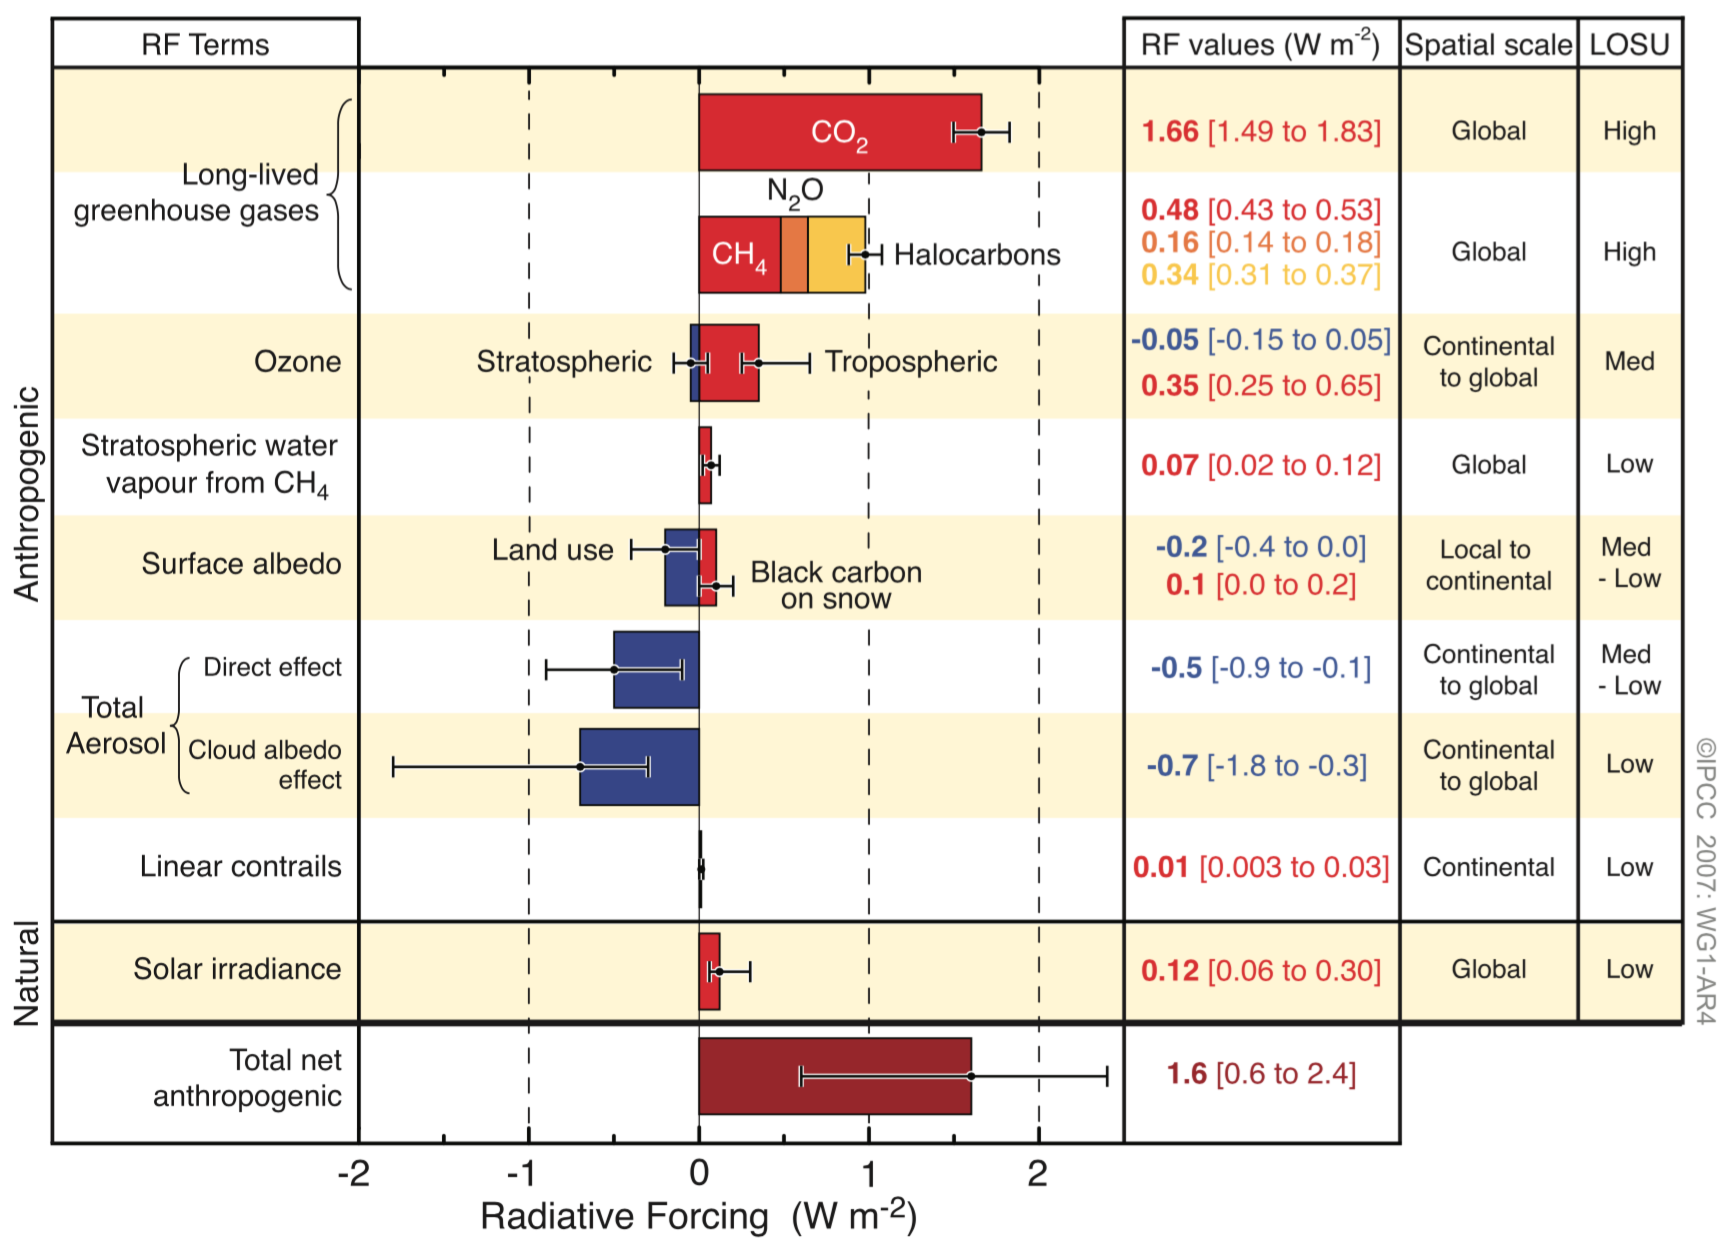
\includegraphics[width=0.8\textwidth,natwidth=1730,natheight=1248]{Fig/Radiative_Forcing.png}
 	\caption{A diagram illustrating the various influences on radiative forcing along with their associated uncertainties. From the 2015 Intergovernmental Panel on Climate Change. The largest contributor to uncertainty is currently aerosols \citep{intergovernmentalpanelonclimatechange:2015fa}.}
 	\label{fig:radforc}
\end{figure}

A major cause of these uncertainties is the necessity for regionally specific aerosol knowledge \citep{intergovernmentalpanelonclimatechange:2015fa}. Aerosol composition and concentration differs greatly with changes in sources and atmospheric conditions. This regional variation translates to variation in direct scattering/absorption and cloud producing potential, leading to both local and global effects on climate. Thus it is important to develop tested, regionally specific models that take into account these variations \citep{cainey:2007jj, simpson:2014}. 

In 1987 the \gls{claw} hypothesis, named after the authors, was defined in the seminal paper `Oceanic phytoplankton, atmospheric sulphur, cloud Albedo and climate'. They proposed a feedback mechanism where stress driven marine biota produced chemicals that influenced cloud cover \citep{charlson:1987fw}. This paper generated a vast body of research involving many disciplines. Dimethyl sulphide (\gls{dms}) is the core chemical responsible for the mechanism and is produced by phytoplankton, and as discovered more recently, coral \citep{raina:2013fj}. As the climate shifts towards increased temperature, regions like the Great Barrier Reef (\gls{gbr}) are increasingly losing coral coverage \citep{hoeghguldberg:1999bi}. It is therefore important to examine the potential effects on climate caused by \gls{dms} producing biota undergoing climate related reduction.

%maybe this needs to be moved to the conclusion?
Modelling \gls{dms} as it is produced, transformed and transported through the atmosphere, in the \gls{gbr} region, will provide needed insight into the mechanisms surrounding \gls{dms}. To do so requires a group of models simulating the different layers of the problem. The bottom most layer is \gls{csiro}'s Conformal-Cubic Atmospheric Model (\gls{ccam}) which provides information such as wind speed and temperature \citep{mcgregor:2005wz}. The middle layer is CSIRO's Chemical Transport Model (\gls{ctm}) which tracks chemical concentrations \citep{cope:2009tz}. The final layer is the Global Model of Aerosol Processes (\gls{glomap}) which simulates aerosol interactions and produces aerosol concentrations. This project will attempt to apply this trio of models, specifically targeting \gls{dms} in the \gls{gbr} region, and to analyse the results with potential for modelling future climate scenarios.

%Understanding the role of the CLAW hypothesis and its current position will provide the necessary foundational knowledge. Looking at the modelling system itself and other modelling studies will give greater clarity in our approach. The pathways \gls{dms} proceeds down to form cloud condensation nuclei (\gls{ccn}) involve complicated chemistry \citep{Barnes:2006ug} and must be examined to ensure we have the best knowledge of current theory to match with the model. Finally, a look at other regionally specific and global large scale studies is needed to form an overview of the problem.

Primarily, it is necessary to understand the role of the atmosphere and its constituents, and where aerosols and \gls{dms} are positioned within it. The pathways \gls{dms} proceeds down to form \gls{ccn} involve complicated chemistry \citep{barnes:2006ug} and must be explored to ensure the modelling mirrors current theory. The unique climatology of the \gls{gbr}, including the mechanism and scale with which coral contributes to \gls{dms}, needs to be established to provide localised inputs for the group of models. Modelling and the models themselves must be understood to ensure they are being applied correctly and to determine if they are sufficient for simulating the \gls{dms} to \gls{ccn} pathway. Finally, researching the method through which \gls{dms} enters the atmosphere, along with previous \gls{dms} to \gls{ccn} modelling attempts, provides insight into the modelling process and what areas of this research area remain unexplored.

%\section{Research Topic}




%!TEX root = Literature_Review_David_Burns.tex

%Todo

% - check your writing style with that writing program
% - get mum to check structure
% - get zoran to check content

%Done

% - put chapters into references
% - read through it for continuity and completeness
% - put in self references where needed


\chapter{Atmosphere}
\label{ch:atmo}

\section{Atmospheric Regions}
\label{sec:atmoreg}

The Earth's atmosphere is split into a number of different layers. The factor governing their division is the sign of the change in temperature with respect to altitude. For example, in \cref{fig:atmolay}, a decrease in temperature ($T$) with an increase in altitude ($z$) in the troposphere occurs up until the tropopause. The difference in temperature gradients between the different levels of the atmosphere prevent mixing from occurring between layers. This occurs as in most circumstances a parcel of air will rise if $\diff{T}{z} < 0$ and fall if $\diff{T}{z} > 0$.

	\begin{figure}[!htb]
	 	\centering
	 	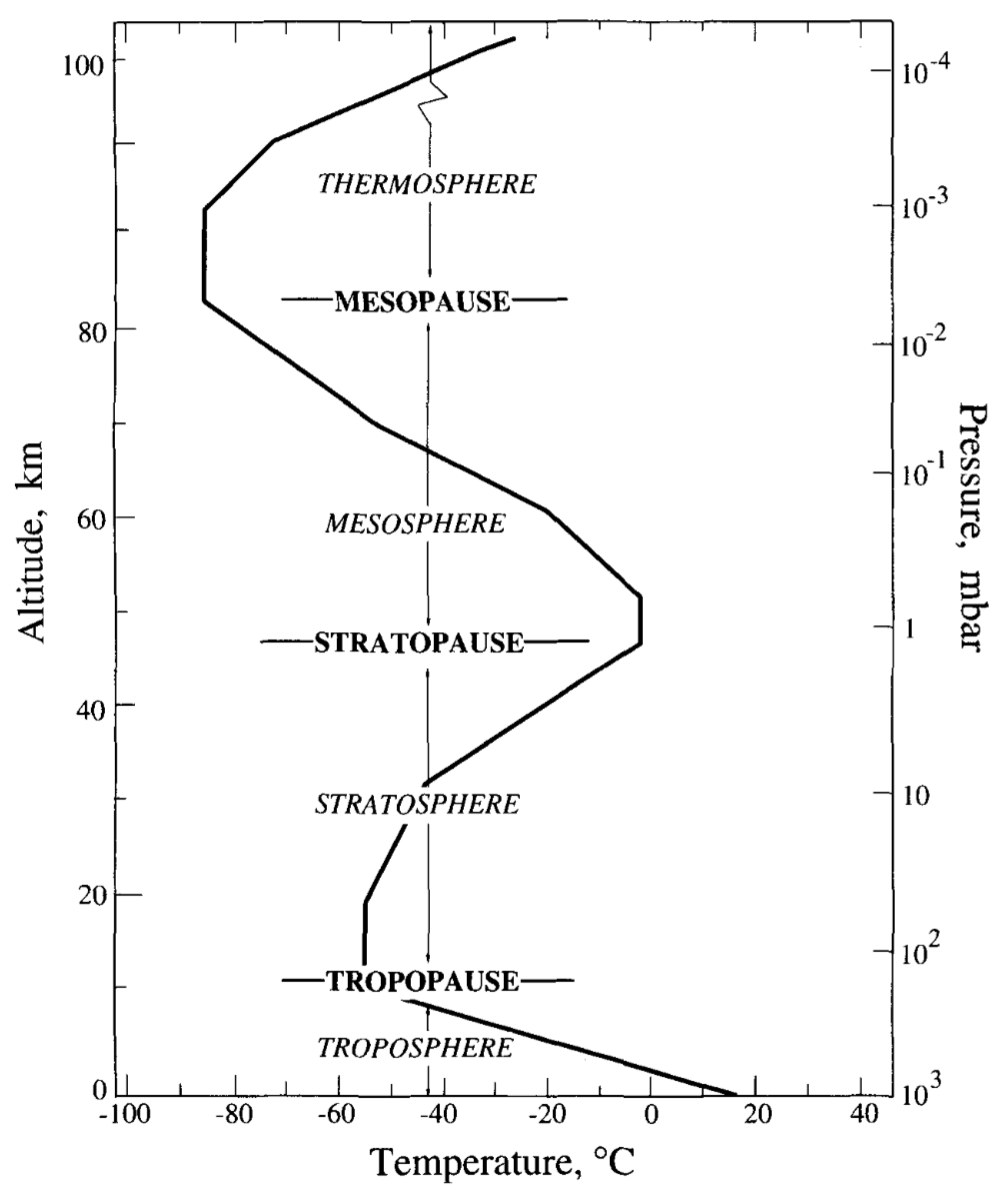
\includegraphics[width=0.8\textwidth,natwidth=1004,natheight=1196]{Fig/Atmosphere_Layers.png}
	 	\caption{The layers of Earth's atmosphere, separated by pauses in temperature change with respect to altitude \citep[p. 7]{seinfeld2012atmospheric}}.
	 	\label{fig:atmolay}
	\end{figure}

\subsection{Troposphere}
\label{subsec:trop}
The troposphere is the lowest level of the atmosphere sitting between $10-15$ \si{\km} above the surface of the Earth. It ends at the tropopause, the first region of constant temperature. The range of altitudes is dependant on time and latitude with the highest region being over the equator, shifting up and down the Earth with its axial tilt \citep[Chapter 1]{seinfeld2012atmospheric}.

The troposphere is an important region as it contains the majority of the atmosphere's mass (approximately \SI{80}{\percent}) and all of its weather. It also contains the highest quantity of water, despite being the smallest region. The layer immediately above the surface of the Earth is called the planetary boundary layer (\gls{pbl}), or marine boundary layer (\gls{mbl}) over the ocean \citep[Chapter 1]{seinfeld2012atmospheric}. The \gls{pbl} varies greatly in height depending on the surface of the Earth it is over, for example, above the Sahara it can be up to \SI{6}{\kilo\meter}, while over tropical oceans it is only \SI{100}{\meter} \citep[Chapter 1]{laing2011introduction}.

There is a short inversion layer in the troposphere that separates the boundary layer and the free troposphere (\gls{ft}) (see \cref{fig:atmolay}). It occurs at only a few hundred metres above tropical oceans \citep{laing2011introduction}. The \gls{ft} is relatively free of aerosols, as the inversion layer prevents mixing with the boundary layer. Thus there is a low aerosol surface area greatly decreasing heterogeneous nucleation. The inversion layer is not always present, and clouds can breach this layer permitting chemicals access into the \gls{ft} from the boundary layer. These conditions promote homogeneous nucleation, which is the formation of new particles \citep[Chapter 8]{seinfeld2012atmospheric}.

\begin{figure}[!htb]
	\centering
	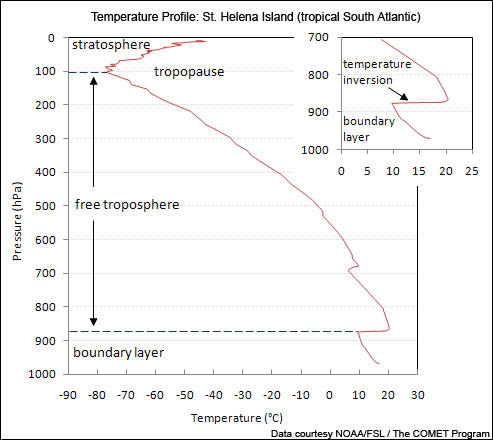
\includegraphics[width=0.8\textwidth,natwidth=493,natheight=440]{Fig/helena_island_skewt.jpg}
	\caption{An example of the separation between \gls{pbl} and \gls{ft} at St. Helena Island. There is an inversion layer present distinguishing the two, however, this obvious separation is not always the case. \citep[Section 1.5.1]{laing2011introduction}}
 	\label{fig:atmolay}
\end{figure}

\section{Relative Humidity and Supersaturation}
\label{subsec:relhum}

The amount of water present in air is usually measured via the relative humidity (\gls{rh}). \gls{rh} is the fraction of the partial pressure of the gas phase water $p_{\text{\tiny H}_2\text{\tiny O}}$ and the saturation vapour pressure for the temperature of the air $p_{\text{\tiny H}_2\text{\tiny O}}^0$, which is the point at which water condenses \citep[Chapter 1]{seinfeld2012atmospheric}. Supersaturation occurs when there is a \gls{rh} greater than \SI{100}{\percent} \citep{rogers1989short}.

\begin{align}
\label{eq:relhum}
	\mathrm{RH} &= 100 \times \frac{p_{\text{\tiny H}_2\text{\tiny O}}}{p_{\text{\tiny H}_2\text{\tiny O}}^0}.
\end{align}

When a parcel of moist air rises in the troposphere the temperature within it decreases which increases the \gls{rh} and a supersaturation can be achieved \citep[Chapter 1]{seinfeld2012atmospheric}. The temperature decreases due to adiabatic expansion. When this occurs water undergoes spontaneous nucleation onto aerosol particles. A seed particle is required for droplet formation to occur; as homogeneous nucleation of water would require a supersaturation far higher than that seen in the atmosphere. \gls{ccn} are the aerosol seeds that droplets form around (see \cref{subsec:ccn}). There is therefore a dependence on the level of supersaturation for an aerosol to act as a \gls{ccn}, which is generally $0.5 - 2$ \si{\percent} \citep[Chapter 6]{rogers1989short}.

% Does the seed particle need to be water soluble?
% i think this is established in the kohler theory paper

\section{Albedo}
\label{sec:albedo}

The albedo of the Earth is given as the ratio between reflected radiation and incident radiation. The amount of light that is not reflected back into space from the surface of the Earth must be absorbed and thus increases the Earth's temperature. Light may be emitted in the infra-red regime as black-body radiation, which either escapes out into space or is absorbed by greenhouse gases in the atmosphere \citep{Lashof:1990wu}. Water acts as a greenhouse gas, but also acts to increase the albedo of the Earth when formed into clouds. A phenomena that alters the amount of light being absorbed by the Earth is said to exhibit radiative forcing \citep{intergovernmentalpanelonclimatechange:2015fa}. Aerosols may cause radiative forcing by either directly reflecting or absorbing light, or by assisting in the formation of clouds \citep{seinfeld2012atmospheric}.


%--------------------------------------------------------------------------------------------------------------------------%
%--------------------------------------------------------------------------------------------------------------------------%

	\section{Aerosols}
	\label{sec:aerosols}

	An aerosol is any solid or liquid particle suspended in a gas. In the troposphere there is an abundance of aerosols present, with a vast range of sizes and composition.

	Aerosols are generally subdivided into modes that indicate their production mechanism. When plotting a property of a large number of particles, such as their number or surface area, against the log of the aerosol diameter, peaks appear at different diameters, which are called modes \citep[Chapter 8]{seinfeld2012atmospheric}. The modes are nucleation, Aitken, accumulation, and coarse. The diameters over which these modes are generally found in the atmosphere can be seen in \cref{fig:aermode}.

	\begin{figure}[!htb]
	 	\centering
	 	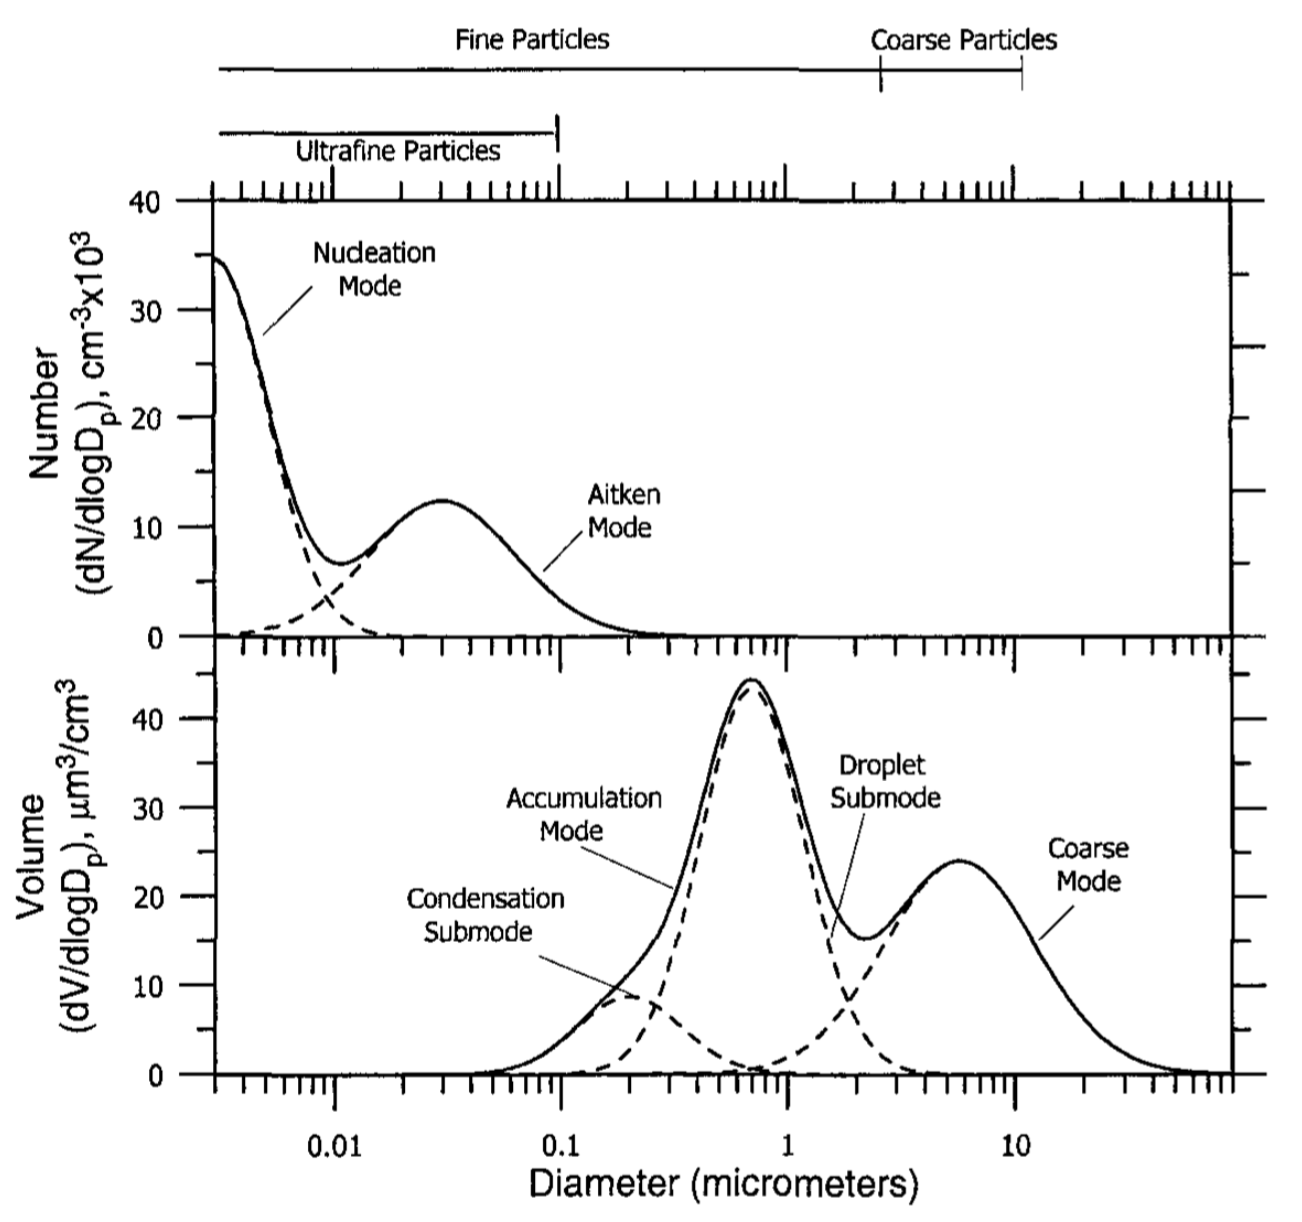
\includegraphics[width=0.8\textwidth,natwidth=1302,natheight=1222]{Fig/aerosolmodes.png}
	 	\caption{A example of the Number and Volume distributions of atmospheric particles indicating the various modes. \citep[Chapter 8]{seinfeld2012atmospheric}}
	 	\label{fig:aermode}
	\end{figure}

	There are many properties of aerosols that can be examined, such as volume, surface area, mass, chemical composition, hygroscopicity, and concentration. For cloud formation the most important characteristics are hygroscopicity, a measure of the particles ability to absorb water, and particle diameter, which governs whether a particle is large enough to act as a \gls{ccn} \citep[Chapter 6]{rogers1989short}. The number, or concentration, of aerosols is important for cloud formation to an extent. If too many \gls{ccn} are present the water vapour concentration may not be high enough to form large droplets \citep[Chapter 22]{seinfeld2012atmospheric}.

	The processes that an aerosol undergoes in the atmosphere dictate some of the modes that appear. The nucleation mode arises from particles homogeneously nucleating from a gas, such as sulphuric acid. The accumulation mode is constructed from particles that have condensed vapour such as water, and/or have grown via coagulation, which occurs when when multiple aerosol particles stick together. The majority of the accumulation mode peak measured in the atmosphere comes from droplet formation in clouds \citep[Chapter 8]{seinfeld2012atmospheric}. This droplet sub-mode can be seen in \cref{fig:aermode}.

	%NSS vs seas salt particles? production and CCN potential?

%--------------------------------------------------------------------------------------------------------------------------%

		\subsection{Particle Formation}

		There are two types of aerosols, primary and secondary. The distinction is based on their method of formation. 

		Primary aerosols are particles that enter the atmosphere directly. In the \gls{mbl} sea salt particles are an example of primary aerosols \citep{quinn:2011iv}.

		Secondary aerosols are aerosols that have formed in the atmosphere via homogeneous nucleation. They begin as gases present in high concentrations, in regions with low concentrations of particles, as heterogeneous nucleation is energetically favourable. Creation of secondary particles are dubbed nucleation events, as the atmospheric conditions required for homogeneous nucleation to proceed are uncommon \citep[Chapter 11]{seinfeld2012atmospheric}. 

		Because nucleation events are rare and localised in time and space they are difficult to simulate, so the percentage of secondary particles on a global scale has a large uncertainty \citep{intergovernmentalpanelonclimatechange:2015fa}. \citet{merikanto:2009iu} modelled global \gls{ccn} production using the \gls{glomap} model and showed that between \SI{31}{\percent} and \SI{49}{\percent} of \gls{ccn} are secondary particles. Approximately \SI{35}{\percent} of these secondary particles were formed in the free and upper troposphere and entrained down into the \gls{mbl} \citep{merikanto:2009iu}.

		% What theory governs nucleation? 
		% Classical vs experimental?

		% \subsection{Marine Aerosols}

		% In the remote ocean aerosols come from a number of different sources. Sea salt is aerosolised through bubble bursting along with primary organic aerosols \citep{cainey:2007jj}. Secondary aerosols are formed from chemicals in the atmosphere, predominantly in the free troposphere \citep{woodhouse:2010ed}. There are also other external sources such as anthropogenic aerosols from shipping or land sources depending on remoteness.

		% The prevalance and effect of aerosols in the remote marine region is the subject of much research and contention \cite{cainey:2007jj}, \citep{quinn:2011iv} \citep{woodhouse:2010ed} \cite{odowd:2007gj}.

%--------------------------------------------------------------------------------------------------------------------------%

		\subsection{CCN}
		\label{subsec:ccn}

		\gls{ccn} are aerosols that are able to act as sites for the heterogeneous nucleation of water. The water droplets continue to grow by precipitating gas phase \gls{h2o} and eventually become massive enough that they fall out of the sky as rain. The formation of clouds requires \gls{ccn}, as the atmospheric conditions for homogeneous nucleation of water are never reached. So \gls{ccn} act as sites for the heterogeneous nucleation of water, forming cloud droplets \citep[Chapter 17]{seinfeld2012atmospheric}. 

		\gls{ccn} are defined for particular supersaturations. This is because whether an aerosol (with a given composition) can act as a \gls{ccn}, is dependant on the supersaturation of the air it is in. The chemical composition of the particle, or it's hygroscopicity, also affect its ability to act as a \gls{ccn}. As this information is not always known, empirical equations are often used to describe the concentration of \gls{ccn}. Take the following equation,
		\begin{align}
			\label{eq:ccnemp}
			\mathrm{CCN}(s) &= cs^k.
		\end{align}
		Here the concentration of \gls{ccn} is given as a power function of supersaturation $s$, where $c$ and $k$ are empirical parameters that conceal the size and composition dependence of \gls{ccn}. The empirical parameters are sampled locationally with $c$ varying between $25 - 3500$ \si{\per\cubic\centi\metre} and $k$ varying between $0.3 - 1.4$ \citep[Chapter 17]{seinfeld2012atmospheric}. If size distributions, composition and supersaturation are known, then K\"{o}hler theory (see \cref{subsec:kohler}) predicts which aerosols may act as \gls{ccn} \citep{rissman:2006ha}.

		\subsubsection{Sources and Sinks for \gls{ccn}}

		There are a number of \gls{ccn} sources. Sea salt is an excellent \gls{ccn} due to its high hygroscopicity \citep{randles:2004ke}. It is also abundant in atmospheric regions above the ocean and coastline. It is aerosolised by bubble bursting and wind shear at the surface of the ocean. 

		Chemicals produced by living organisms can pass through a series of chemical reactions and a subsequent nucleation event to produce \gls{ccn}. An example of this is \gls{dms} produced by phytoplankton, which is further explored in \cref{ch:dms}. An alternative to \gls{dms} derived organic aerosols is dissolved organic matter from dying biota collected at the surface that is aerosolised through bubble bursting \citep{bigg:2007er}. 
		
		There are also a number of anthropogenic sources of \gls{ccn}, however, in the Great Barrier Reef region, only sources from shipping exhaust are likely to be of consequence \citep{fischer2012atmospheric}.

		Aerosols are readily removed from the atmosphere by rainfall and this is even more apparent for \gls{ccn} as they provide the site of droplet formation. Rain also collects aerosols as the droplets fall \citep{rogers1989short}. Deposition onto other aerosol particles is another way in which \gls{ccn} may be removed while it is also possible for aerosols to deposit directly onto the surface of the Earth \citep[Chapter 9]{seinfeld2012atmospheric}.

		\subsection{K\"{o}hler Theory}
		\label{subsec:kohler}
			K\"{o}hler theory was first described in a paper written by the theory's namesake Hilding K\"{o}hler \citep{kohler:1936dq}. It provides a model for the growth of existing particles by heterogeneous nucleation. There are two forces influencing this behaviour, the attraction of a molecule's neighbours (the Kelvin effect), and the concentration of the solution (the solute effect) \citep{rogers1989short}.

			For a particle of diameter $D_p$, the log of the ratio between the water vapour pressure of a droplet and a flat surface is given as a function of the molecular mass of water $M_w$, the surface tension $\sigma_w$, the gas constant $R$, the temperature $T$, the water density $\rho_w$, and the number of moles of the solute $n_s$.
			\begin{align}
				\ln \left(\frac{p_w(D_p)}{p^\circ}\right) &= \frac{4 M_w \sigma_w}{R T \rho_w D_p} - \frac{6 n_s M_w}{\pi \rho_w D_p^3}.
				\label{eq:kohler}
			\end{align}

			Substituting in the known constants produces $\frac{4 M_w \sigma_w}{R T \rho_w} \approx \frac{0.66}{T}$ and $\frac{6 n_s M_w}{\pi \rho_w} \approx \frac{\num{3.44e13} v m_s}{M_s}$ with units \si{\micro\meter} \citep[p. 770]{seinfeld2012atmospheric}. The moles of solute $n_s$ is given by the ratio between the number of ions per molecule $v$, the solute particle mass $m_s$ and the solute molar mass $M_s$. Substituting into \cref{eq:kohler} gives,
			\begin{align}
				\frac{p_w(D_p)}{p^\circ} &= e^{\frac{0.66}{T D_p}} e^{-\frac{\num{3.44e13} v m_s}{M_s D_p^3}}.
				\label{eq:kohlerapp}
			\end{align}
			Here the first exponential term represents the Kelvin effect and the second represents the solute effect.

			Plotting \cref{eq:kohlerapp} produces K\"{o}hler curves that show, for an initial dry particle size, the required supersaturation for particle growth to occur even as the particle itself grows and changes concentration. An example of K\"{o}hler curves for different seed diameters of ammonium sulphate \gls{amsu} can be seen in \cref{fig:kohleras}. Here, \cref{eq:kohlerapp} has been plotted with $v = 3$, $M_s = \SI{132.14}{\gram\per\mole}$.

			\begin{figure}[!htb]
			    \centering
			    \includegraphics[width=0.8\textwidth]{Fig/as_Kcurve.eps}
			    \caption{The K\"{o}hler curves for ammonium sulphate \gls{amsu} for three dry diameters $0.05$, $0.1$, $0.5$ \si{\micro\meter} using approximations from \citet[p. 770]{seinfeld2012atmospheric} }
			    \label{fig:kohleras}
			\end{figure}

			% 'maybe we shouldnt bother with the figure below, we would need a whole bunch more explanation for where the equations come from for it :('

			% \begin{figure}[htpb]
			%     \centering
			%     \includegraphics[scale=0.43]{Fig/as_GvH.eps}
			%     \caption{Growth factor as a function of Relative Humidity for Ammonium Sulphate $(\mathrm{NH}_4)_2\mathrm{SO}_4$ for dry diameter $0.03$ \SI{}{\micro\meter} using approximations from \citet{tang1994water}. Data for comparison comes from \citet{Hameri:2000tc}.}
			%     %\label{fig:}
			% \end{figure}

			There are a number of variations to the general form of the K\"{o}hler curve equation that deal with alternate conditions, such as insoluble seed particles, and mixes of soluble and insoluble seeds \citep[Chapter 17]{seinfeld2012atmospheric}.


%!TEX root = Literature_Review_David_Burns.tex

%Todo

% - send to mum for editing
% - send to zoran to check content

%Done

% - Get rough version of totally complete chapter
% - remove all the '' reminders and any quotations
% - trim down some of these sections, just because you reviewed the paper intensely doesnt mean you need it all
% - put in self referencing
% - prep final draft


\chapter{Dimethyl Sulphide}
\label{ch:dms}

Dimethyl sulphide (\gls{dms}) is a naturally produced chemical that has been theorised to influence cloud coverage and potentially act as a negative feedback mechanism for climate change \citep{charlson:1987fw}. \gls{dms} enters the atmosphere and goes through an array of chemical reactions to produce sulphuric acid (\gls{h2so4}) \citep{barnes:2006ug}, which may then nucleate into aerosols that can act as \gls{ccn}. Measurements of aerosols in the atmosphere, particular remote marine areas show a large percentage being of the non-sea salt sulphate variety, potentially sourced from \gls{dms} \citep{o1997marine}.  

%--------------------------------------------------------------------------------------------------------------------------%
%--------------------------------------------------------------------------------------------------------------------------%

	\section{Chemistry}
	\label{sec:chem}

	The chemical processes that \gls{dms} and dimethyl sulfoxide \gls{dmso} undergo in the atmosphere are extremely complicated with many competing pathways (see \cref{fig:dmspath}). \citet{barnes:2006ug} have reviewed the extensive literature on this subject, with great detail. They split the problem into three sections, the first, \gls{dms} reactions and products, the second, \gls{dmso} reactions and products, and the third, multiphase chemistry of the \gls{dms} pathways.

	The reaction processes for \gls{dms} are reactions with the \gls{oh} radical, the \gls{no3} radical, and with Halogen Atoms and Oxides.  During the day the dominant reaction is the addition pathway through \gls{oh}, while at night it is the abstraction pathway through \gls{no3} as seen in \cref{fig:dmspath} \citep{barnes:2006ug}. Pathways involving halogen species are generally ignored in modelling due to low availability, though levels of hypobromite high enough to be influential have been measured in the troposphere \citep{platt2003role}.

	\begin{figure}[!htb]
	 	\centering
	    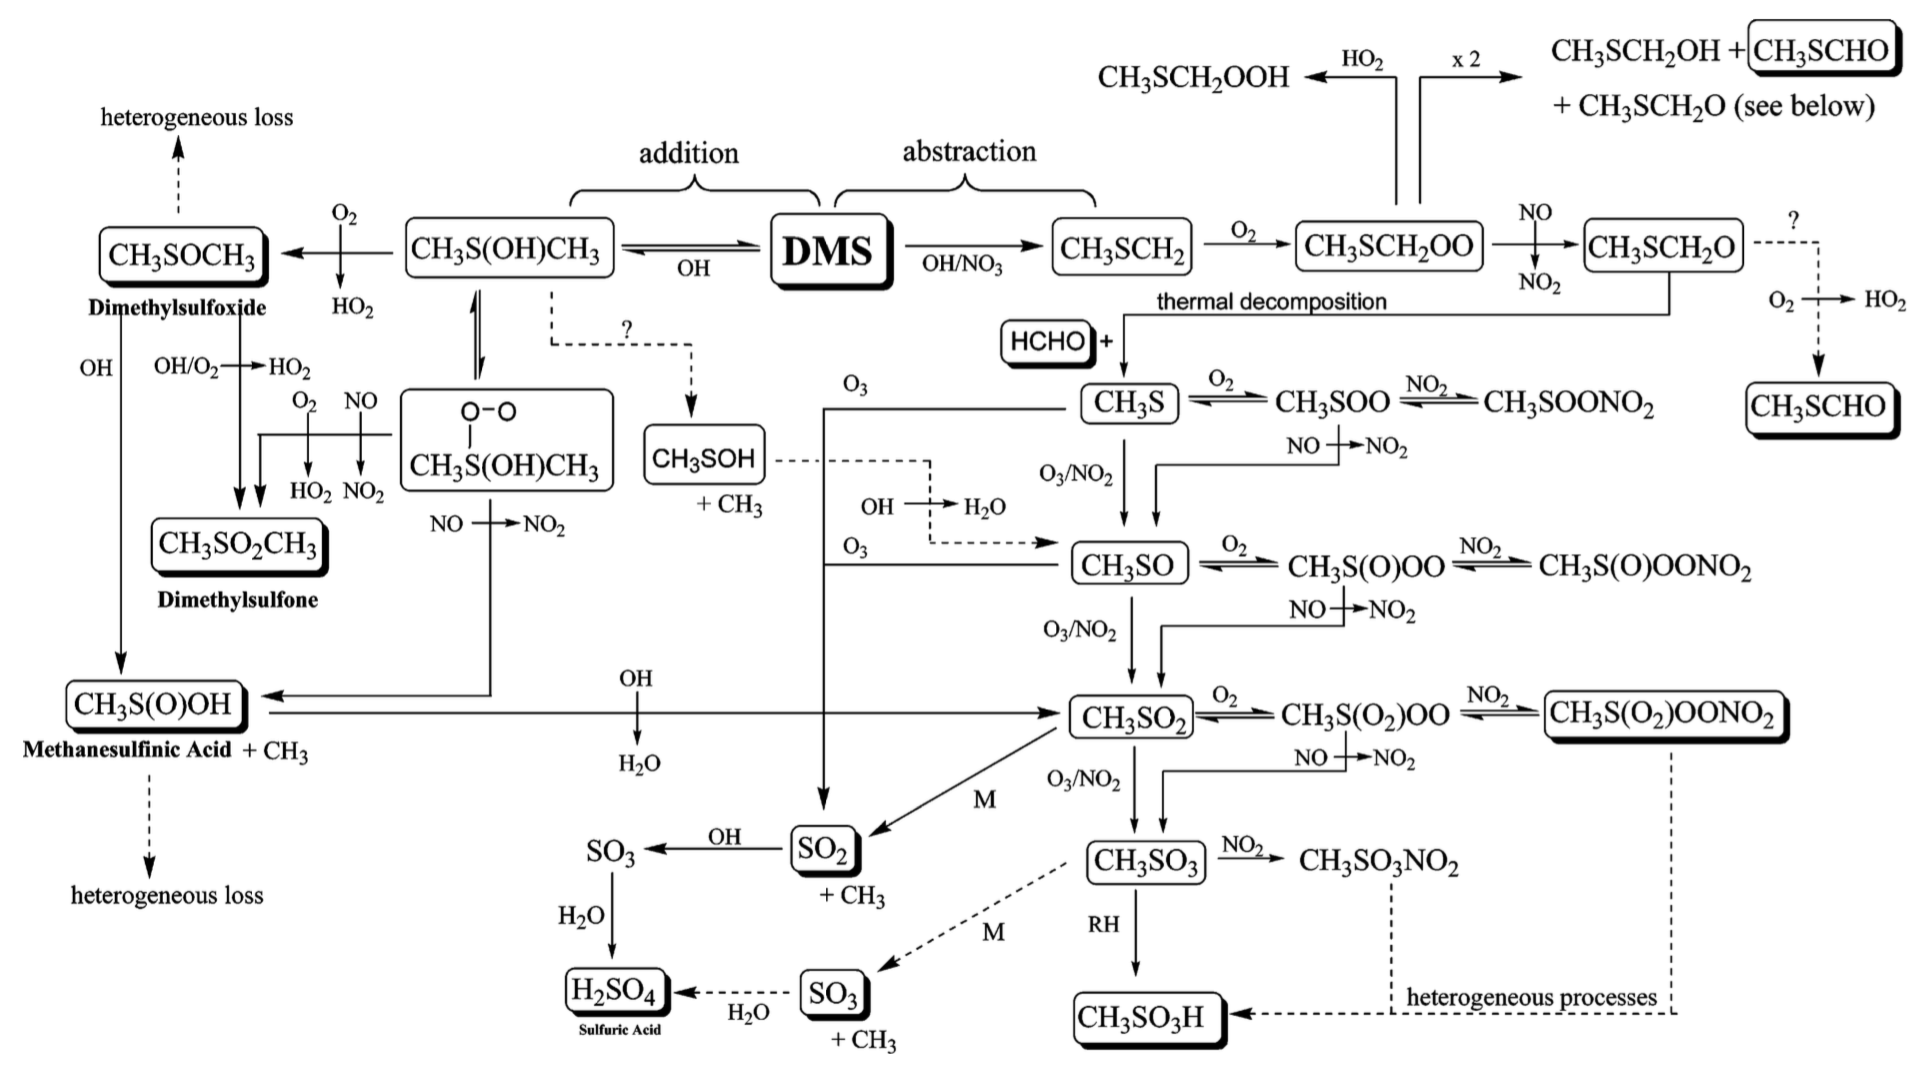
\includegraphics[width=0.95\textwidth,natwidth=1924,natheight=1068]{Fig/dms_Pathway.png}
	    \caption{The reaction scheme for \gls{dms} oxidised by \gls{no3} and \gls{oh} radicals \citep{barnes:2006ug}.}
	    \label{fig:dmspath}
	\end{figure}

	\gls{dmso} appears to be the major product of \gls{dms} oxidation in the atmosphere. Its reactions are the same as for \gls{dms} listed above. The atmospheric lifetimes calculated indicate that \gls{oh} radicals dominate reactions for \gls{dmso} \citep{barnes:2006ug}. Methane sulphinic acid (\gls{msia}) is a product of this reaction, which goes on to form methane sulphonic acid (\gls{msa}). \gls{dmsot} is also a product of this reaction and was considered the most prevalent pathway, but \citet{barnes:2006ug} found instead that the \gls{msia} pathway heavily dominates. \gls{sot} is the largest possible outcome of \gls{msa} oxidation.

	\subsection{Multiphase Chemistry}
	\label{subsec:multchem}

	The pathways examined in the preceding section are for gas phase reactions. However the atmosphere also contains liquid water in the form of droplets leading to aqueous phase reactions. The difference between gas and aqueous phase reactions is largely due to the availability of \gls{h2o} and \gls{hp} \citep{barnes:2006ug}. A combination of the two, multiphase chemistry, is needed. Interestingly, \gls{dms} is not as soluble in water as \gls{dmso}, \gls{dmsot}, \gls{msa} and \gls{msia} so its multiphase reactions are not as important.

	\citet{barnes:2006ug} have analysed the multiphase chemistry of all five chemicals and recommend that modellers implement the multiphase chemistry they have illustrated. They include a list of aqueous phase rate coefficients for the five chemicals of major interest, though do not consider a coupling of the gas and aqueous-phase systems necessary. \citet{jacob2000heterogeneous} provides a method for calculating chemical uptake by aerosols, while Henry's law is recommended for calculating concentrations, as an approximation.
	

%--------------------------------------------------------------------------------------------------------------------------%
%--------------------------------------------------------------------------------------------------------------------------%

	\section{Dimethyl Sulphide, Aerosols and the Environment}
	\label{sec:daande}


%--------------------------------------------------------------------------------------------------------------------------%

		\subsection{The CLAW Hypothesis}
		\label{subsec:clawhyp}

		\begin{figure}[!htb]
	 	    \centering
	 	    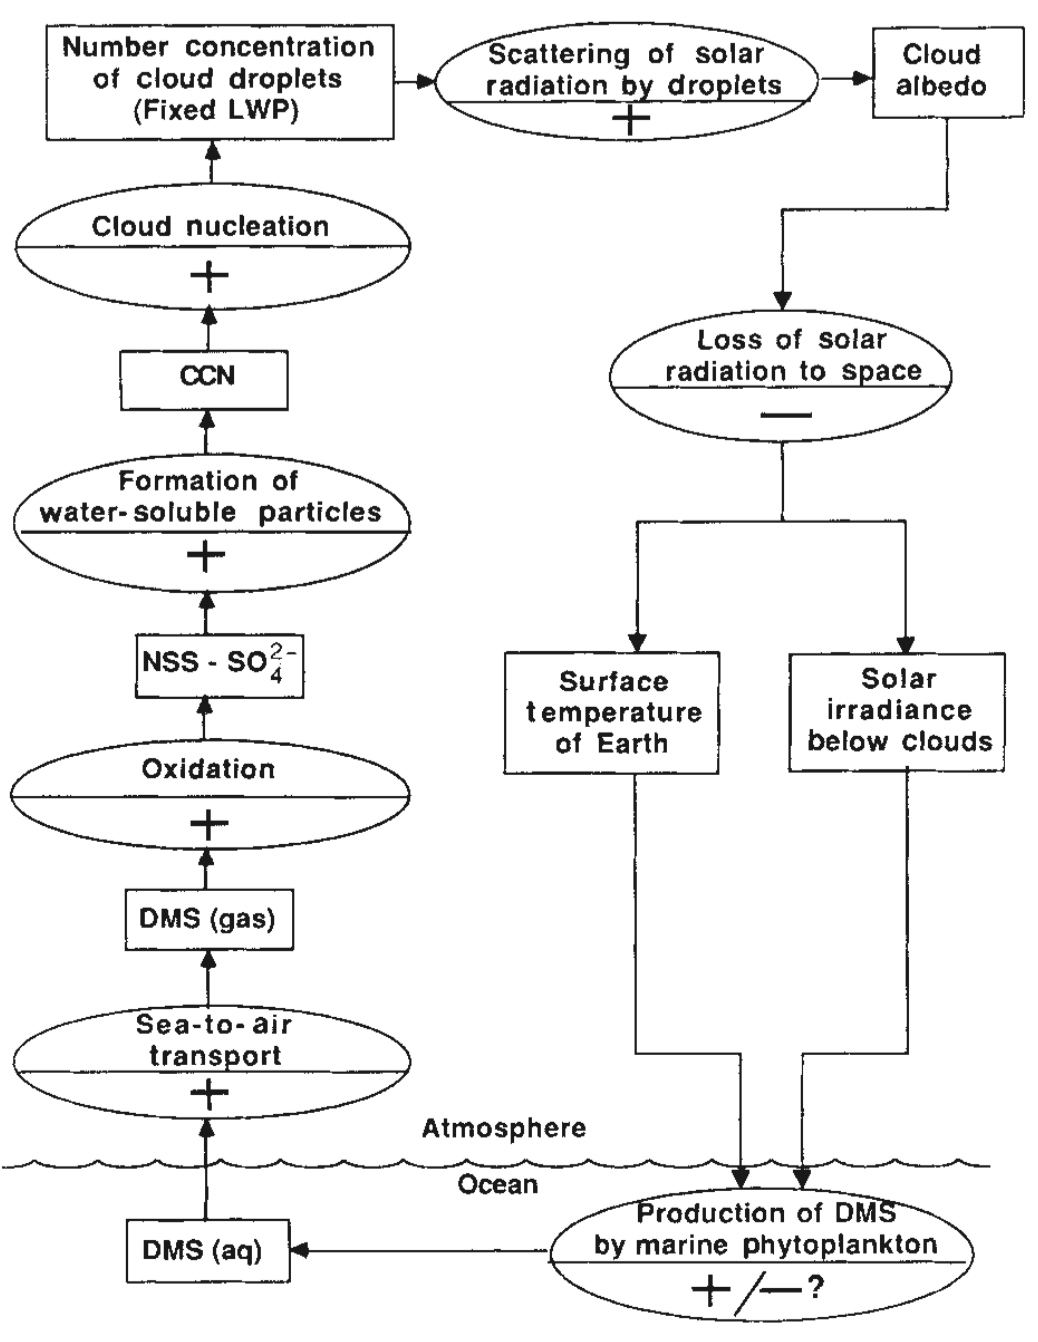
\includegraphics[width=0.7\textwidth,natwidth=1038,natheight=1342]{Fig/Original_Claw_Cycle.png}
	 	    \caption{The original feedback loop diagram describing the \gls{claw} hypothesis postulated in the paper by \citet{charlson:1987fw}. Rectangles are measurables, ovals are processes. The sign indicates the effect a positive change in the previous rectangle has on the next rectangle. The appearance of both signs in the production of \gls{dms} oval reflects the author's uncertainty of this particular effect. If it is positive, then the diagram describes a negative feedback loop, stabilising the climate.}
	 	    \label{fig:origclaw}
	 	\end{figure}

		In the \gls{claw} hypothesis \gls{dms} produced by phytoplankton in the ocean was considered as the precursor for \gls{ccn} in the \gls{mbl}. The \gls{ccn} produced were investigated for their cloud producing properties and the subsequent change in planetary albedo. The feedback loop, as seen in \cref{fig:origclaw}, was closed by linking the \gls{dms} precursor dimethylsulphoniopropionate (\gls{dmsp}) to a survival trait of the phytoplankton.

		Anthropogenic sources were ignored as the regions the hypothesis focussed on were remote, while other natural gaseous sulphur producers were considered insignificant. The purpose for phytoplankton's production of \gls{dms} was suggested to be from \gls{dmsp}, used in osmo-regulation and the cycle for methionine \citep{vairavamurthy:1985gw}. The highest flux of \gls{dms} from the ocean to the atmosphere was concluded to occur in the most saline, hottest and sunlit areas. The formation of sub-micrometer \gls{nss} sulphate particles was attributed to the oxidation of \gls{dms} by hydroxide. Other reactions removing \gls{dms} to non \gls{ccn} forms were considered too low to have a significant effect. From here it was concluded that increases in \gls{dms} flux from the ocean directly increased the number of \gls{ccn} present in the form of NSS sulphate aerosols \citep{charlson:1987fw}.

		\citet{charlson:1987fw} attempted to establish \gls{nss} sulphate as the prominent \gls{ccn} in the remote marine atmosphere and that higher concentrations increased or altered the reflective properties of cloud cover and thus albedo. \gls{nss} sulphate particles derived from \gls{dms} were considered to be in the right size range and have the correct properties for acting as \gls{ccn}. They used a model developed by \citet{twomey:1977} to predict the change in albedo from the change in the number of \gls{ccn}. By keeping the water content constant and increasing the number of \gls{ccn}, the mean radius of the droplets formed decreased. However the overall surface area of the droplets increased, thereby increasing cloud albedo. The model was used along with top of cloud satellite data to predict a change of $0.016$ to planetary albedo from a \SI{30}{\percent} increase in \gls{ccn}.

		The final part of the loop involved the \gls{dmsp} production mechanism and an attempt to link phytoplankton species that emit large amounts of \gls{dmsp} with increased survival. A number of possible explanations were put forward, such as increased ocean salinity during ice ages, as \gls{dmsp} protects against dessication. The resulting accidental formation of \gls{ccn} may have acted as a further survival mechanism. This completes the hypothesis that a negative feedback mechanism exists where increases in the Earth's temperature increases planetary albedo which then decreases the Earth's temperature \citep{charlson:1987fw}.

		%The \citet{Charlson:1987fw} paper helped to establish what is now known as Earth Systems Science, and much inter-disciplinary collaboration as the various aspects of the feedback mechanism lie in different areas of science.

		An analysis of aerosol data collected at Cape Grim in Tasmania was one of the first attempts to experimentally validate the \gls{claw} hypothesis \citep{ayers:1991gd}. \citet{ayers:1991gd} compared concentrations of methane sulphonic acid (\gls{msa}) and concentrations of \gls{ccn}. \gls{msa} was considered a relevant surrogate for \gls{dms} in the absence of long term \gls{dms} data. The results showed a correlation between \gls{msa} and \gls{ccn} concentrations along with seasonal dependence. Interestingly, there was a period during winter where \gls{msa} dropped close to zero while \gls{ccn} did not, indicating the presence of an unknown \gls{ccn} source. The relationship between \gls{msa} and \gls{ccn} was found to be non-linear. This experiment showed that the production of \gls{ccn} from phytoplankton aspect of the \gls{claw} hypothesis was at least plausible.


%--------------------------------------------------------------------------------------------------------------------------%

		\subsection{Post-CLAW Research}
		\label{subsec:postclaw}

		The \gls{claw} hypothesis has prompted a large amount of research and experimentation. \citet{quinn:2011iv} explored this research and formed the view that the hypothesis has been invalidated. The three core elements of the \gls{claw} hypothesis were identified as follows: a significant proportion of \gls{ccn} in the \gls{mbl} must be \gls{dms} derived, changes in \gls{dms} derived \gls{ccn} cause changes to cloud albedo, and \gls{dms} production is affected by ocean surface temperatures and solar radiation changes due to cloud albedo \citep{quinn:2011iv}. The final cycle proposed by \citet{quinn:2011iv} can be seen in \cref{fig:quinncyc}.

		\citet{quinn:2011iv} identified two primary \gls{ccn} competitors, sea salt particles and primary organic particles. A significant amount of \gls{mbl} \gls{ccn} were found to have a sea salt nucleus. Experiments where particles were heated past \SI{600}{\celsius} reported \SI{20}{\percent} refractory particles sourced at \SI{400}{\metre} across the Atlantic, and \SI{40}{\percent} aboard a research ship in the north-east Atlantic. Sea salt particles are likely to be the only refractory particles present \citep{o1993physicochemical}. Sea salt particles were also found to make up \SI{60}{\percent} of evaporated cloud droplets. The difference in these percentages is because sea salt particles act as \gls{ccn} at lower supersaturations \citep{tang1997thermodynamic}.

		Primary organic particles are aerosolised through the same mechanism as sea salt, but the constituents come from the detritus of organisms which collects on the ocean surface. The larger organic particles may break up in the atmosphere due to UV exposure or acidification. According to measurements recorded in the North Atlantic ocean, mass concentration of these particles increased during bloom periods \citep{o2004biogenically}. Organic particles (and sea salt) may also scavenge \gls{dms} products, which removes their effect on \gls{ccn} concentrations, if the scavenging particle was already acting as a \gls{ccn}. Due to the seasonal nature of primary organic particles, they may account for some of the seasonal relationship originally found by \citet{ayers:1991gd}, between \gls{dms} and \gls{ccn} concentrations.

		For the remaining \gls{dms} derived particles, direct nucleation of \gls{dms} products likely occurs at the top of clouds, in the \gls{ft}. Clouds remove existing particles in this region, which decreases the available surface area, and promotes homogeneous nucleation \citep{perry1994further}. Deep convective clouds also move \gls{dms} up into the \gls{ft} \citep{clarke1998particle}. The faster winds present in the \gls{ft} would move the particles away from the \gls{dms}'s origin, breaking the localisation required for the feedback loop. \citet{quinn:2011iv} argues that the majority of \gls{dms} derived particles present in the \gls{mbl} are from this process.

		\citet{cainey:2007jj} similarly identified three main ideas through which the feedback mechanisms of the \gls{claw} hypothesis have been diminished. These are: the effectiveness of \gls{dms} to become \gls{ccn}, the prevalence of sea salt particles in the \gls{ccn} size range, and the direct aerosolisation of organic particles from the ocean surface through bubble bursting.

		\begin{figure}[!htb]
	 	    \centering
	 	    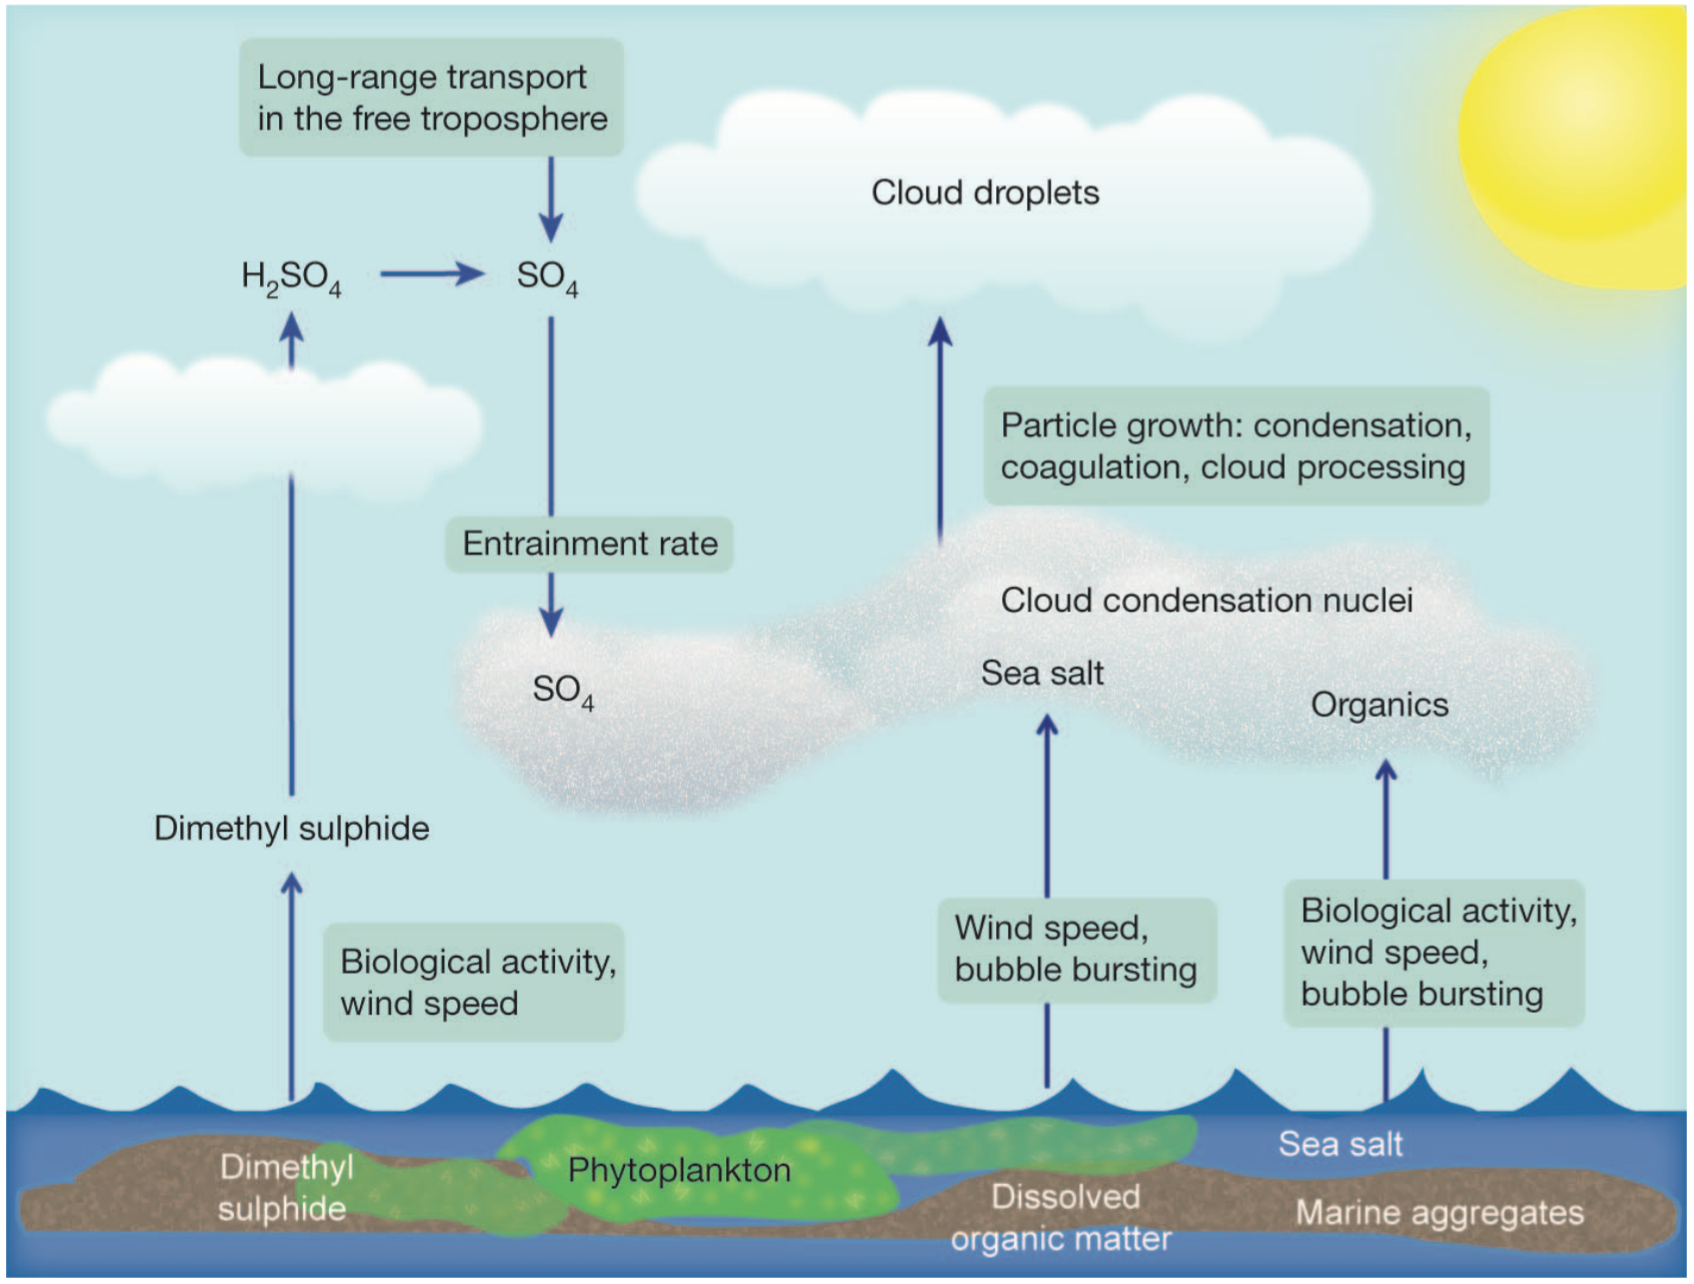
\includegraphics[width=0.8\textwidth,natwidth=1694,natheight=1284]{Fig/quinncycle.png}
	 	    \caption{An updated cycle for \gls{ccn} production in the \gls{mbl}. Major changes to the cycle in \cref{fig:origclaw} are nucleation in the \gls{ft} driven by clouds, and the presence of sea salt and primary organic aerosols \citep{quinn:2011iv}.}
	 	    \label{fig:quinncyc}
	 	\end{figure}

		The effect that aerosols have on cloud albedo is more complicated than the direct relationship proposed in the original \gls{claw} hypothesis \citep{quinn:2011iv, cainey:2007jj}. An increase in cloud albedo can be countered by a decrease in cloud fraction through improved entrainment of sub-saturated air around the cloud \citep{zuidema2008shortwave}. \citet{charlson:1987fw} predicted a \SI{1.3}{\celsius} decrease in surface temperature for a \SI{30}{\percent} increase in \gls{ccn}. As the extra \gls{ccn} are unlikely to be entirely \gls{dms} derived, the required increase in \gls{dms} flux would need to be very high, around \SI{300}{\percent} according to values modelled by \citet{woodhouse:2010ed}.

		An alternative action through which \gls{dms} derived sulphur compounds are removed, and thus prevented from becoming \gls{ccn} directly, is through heterogeneous nucleation onto existing particles \citep{cainey:2007jj}. Such an action may work to alter the chemistry of the particle and thus the albedo of the clouds formed from them. This may provide an alternate way for \gls{dms} to affect climate. 

		\citet{quinn:2011iv} advise that the \gls{claw} hypothesis should be retired, but acknowledge its impact in developing this area of science. Other mechanisms of climate regulation may still be present, such as sea salt particle concentration increases with wind speed, and primary organic particles with biological production. \citet{cainey:2007jj} take a more compromising stance, advising that research into the \gls{claw} hypothesis is still on-going and current results need to be fully implemented in modelling.


%--------------------------------------------------------------------------------------------------------------------------%
%--------------------------------------------------------------------------------------------------------------------------%
%Zoran said to remove :)
% \section{Links to experimentation 'rename'}

% 'do i even need this section?'

% how do you actually measure DMS or SO2? gas chromotography?
% From seawater collected.
% "DMS was trapped on a gold tube attached to the top of the purge chamber. These tubes were sealed with parafilm, labelled and analysed by gas chromatography for DMS at the laboratory (Curran et al. 1998)"
% \citep{Jones:2005ez}

% What is gas chromotography?

% What is pmf?
% Mark at CSIRO spoke about a technique called positive matrix factorisation which can give an estimate of a single chemical or aerosols source fractions. Write a bit about it in here.

% Matt said there is a website containing up to date chemical reaction rates in the atmosphere. Have a look at it and supply a list of the ones we are interested here.

% Experimentation can go either way with this model, and should probably have both. There are some things that we need measured to make the inputs of the model more accurate, particularly DMS surface flux around the \gls{gbr}. So establish a number of parameters that you think the model may predict, that can be checked with experimentation. Then list a number of paramaters that you would want tested to use as inputs for future runs of the model. Maybe even create a flow diagram of the modelling <-> experimentation structure.



%!TEX root = Literature_Review_David_Burns.tex

%Todo

% - send to mum for editing
% - send to zoran to check content

%Done

% - Get rough version of totally complete chapter
% - remove all the '' reminders and any quotations
% - put in self referencing
% - prep final draft
% - print and self edit

\chapter{The Great Barrier Reef}
\label{ch:gbr}

	The Great Barrier Reef (\gls{gbr}) is the world's largest organic structure. The marine park encompassing it is \SI{344400}{\square\km} (see \cref{fig:gbrboundary}), of which around \SI{6}{\percent} is comprised of \SI{2900}{} separate coral reefs \citep{borthwick:2006uv}.

	\begin{figure}[!htb]
	    \centering
	    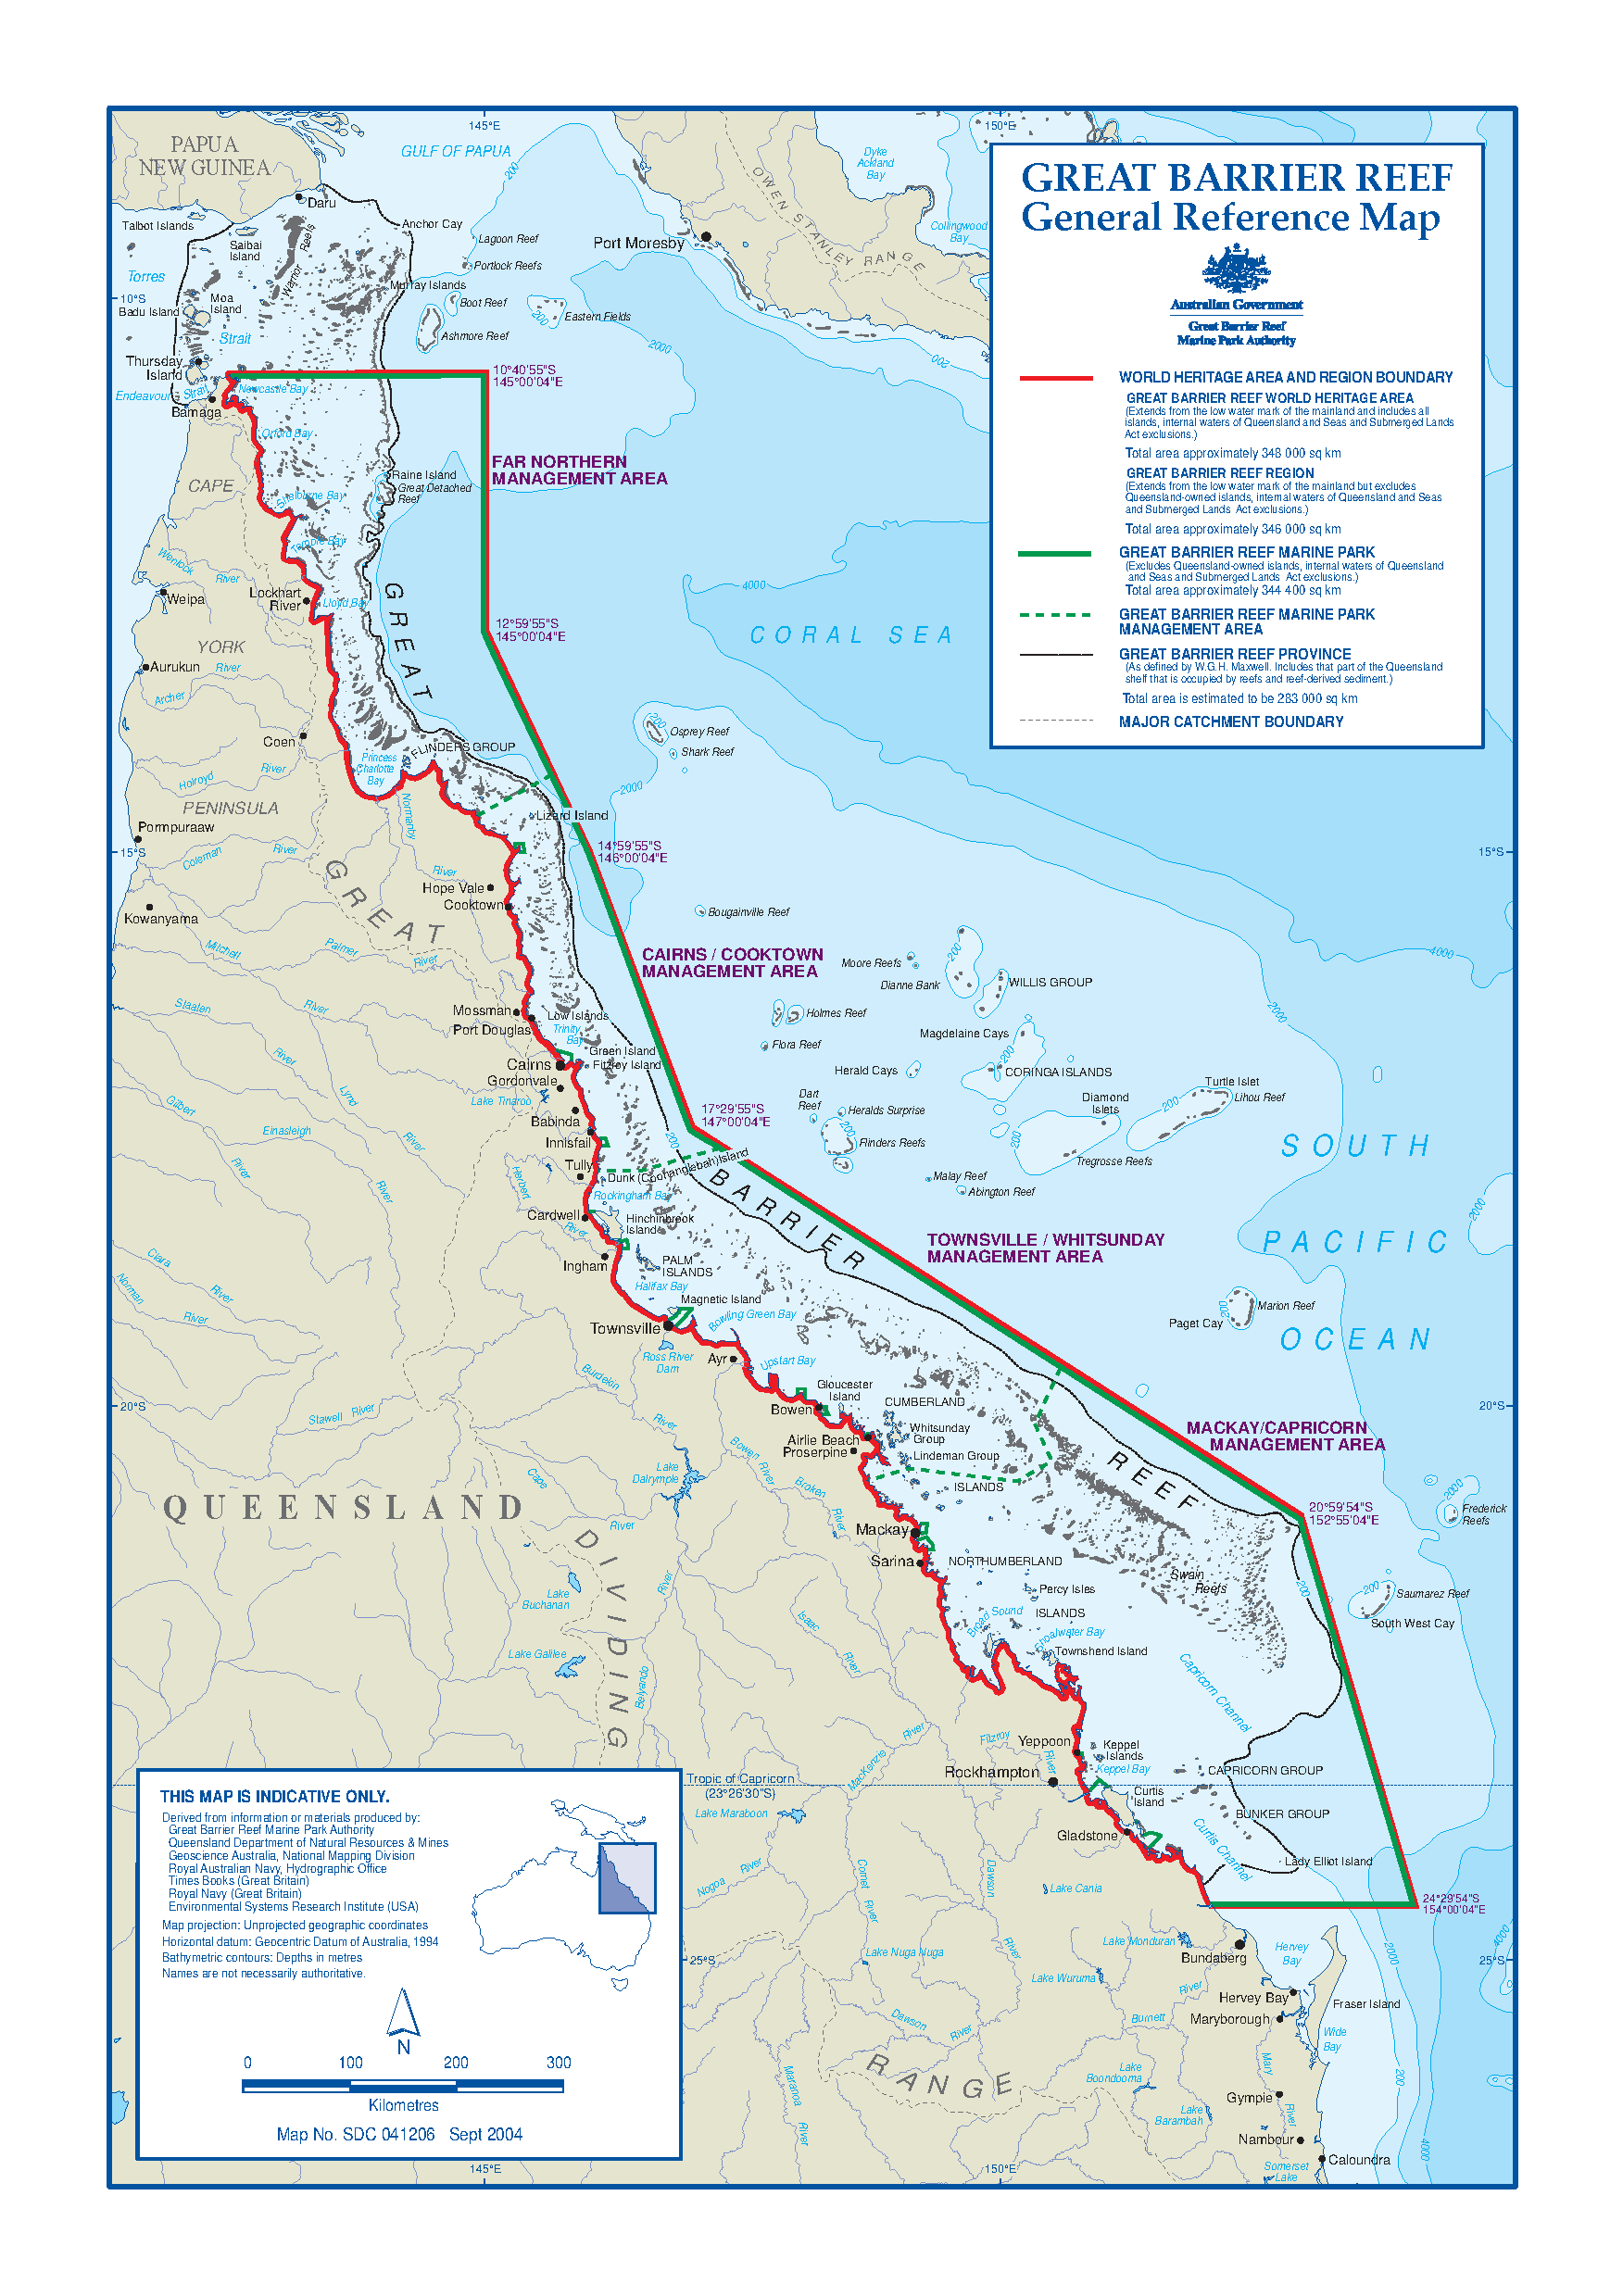
\includegraphics[width=0.9\textwidth,natwidth=787,natheight=1135]{Fig/GBR_map.pdf}
	    \caption{The boundary of the Great Barrier Reef Marine Park illustrating the extent of its coverage along the Queensland coast \citep{borthwick:2006uv}.}
	    \label{fig:gbrboundary}
	\end{figure}

	Climate change is causing an increase in sea surface temperature (\gls{sst}), which effects coral survival in the \gls{gbr} \citep{hoeghguldberg:1999bi}. Stresses associated with changing conditions may also impact coral's production of \gls{dms} \citep{raina:2013fj}.

	Satellite imagery has been used to try and establish a link between \gls{sst} and cloud coverage in the \gls{gbr}. \citet{leahy:2013en} found relationships where changes in \gls{sst} was responsible for changes in cloud cover, but also that cloud cover was responsible for changes in \gls{sst}. Both were found to have a three day delay. The \gls{sst} to cloud cover correlation implies a negative feedback mechanism for cloud formation, with \gls{dms} produced by stressed coral mentioned as a possible source \citep{leahy:2013en}.

%------------------------------------------------------------------------------------------------------------------
%------------------------------------------------------------------------------------------------------------------

	\section{Coral DMS Production}
	\label{subsec:coraldms}

	While the \gls{claw} hypothesis was based only on phytoplankton as a producer of \gls{dms}, phytoplankton are not the only organisms responsible for its production. \gls{dmsp} production by coral is another source. Research has been performed on the effects of ocean temperature changes \citep{jones2007factors}, and the role of Symbiodinium (their algal endosymbiont) in \gls{dmsp} production \citep{raina:2013fj}. \gls{dmsp} is converted to \gls{dms} by bacteria in the ocean \citep{todd2007structural}.

	Separate research on \gls{dmsp} production by Symbiodinium, and adult coral, had previously shown a discrepancy in total \gls{dmsp} production. Experimentation on the larval phase of coral yet to be inhabited by Symbiodinium has shown that coral larvae produce \gls{dmsp} independently \citep{raina:2013fj}. \gls{dmsp} concentration from coral was also found to be two times higher than that produced by benthic algae common to the \gls{gbr} \citep{raina:2013fj}. 

	%Coral was raised in the dark and DNA marker tests were used to rule out the presence of Symbiodinium or other algae. NMR was used to observe \gls{dmsp} concentration. \gls{dmsp} concentration was found to be two times higher than that produced by benthic algae common to the \gls{gbr}. The concentration also increased over time ruling out any carry over effect.

	An increase in temperature has been found to result in an increase in coral \gls{dmsp} production (see \cref{fig:coralstressdms}). \gls{dms} is known to have antioxidative effects, implying that increased \gls{dmsp} production is a defence against damage caused by heat stress. Adult colonies whose Symbiodinium was destroyed by heat stress also produced increasing levels of \gls{dmsp} with increasing temperatures. Prior to \citet{raina:2013fj}, it was assumed that increasing temperatures killing off the Symbiodinium would quickly decrease \gls{dmsp} production. This no longer appears to be the case.

	\begin{figure}[!htb]
	 	\centering
	    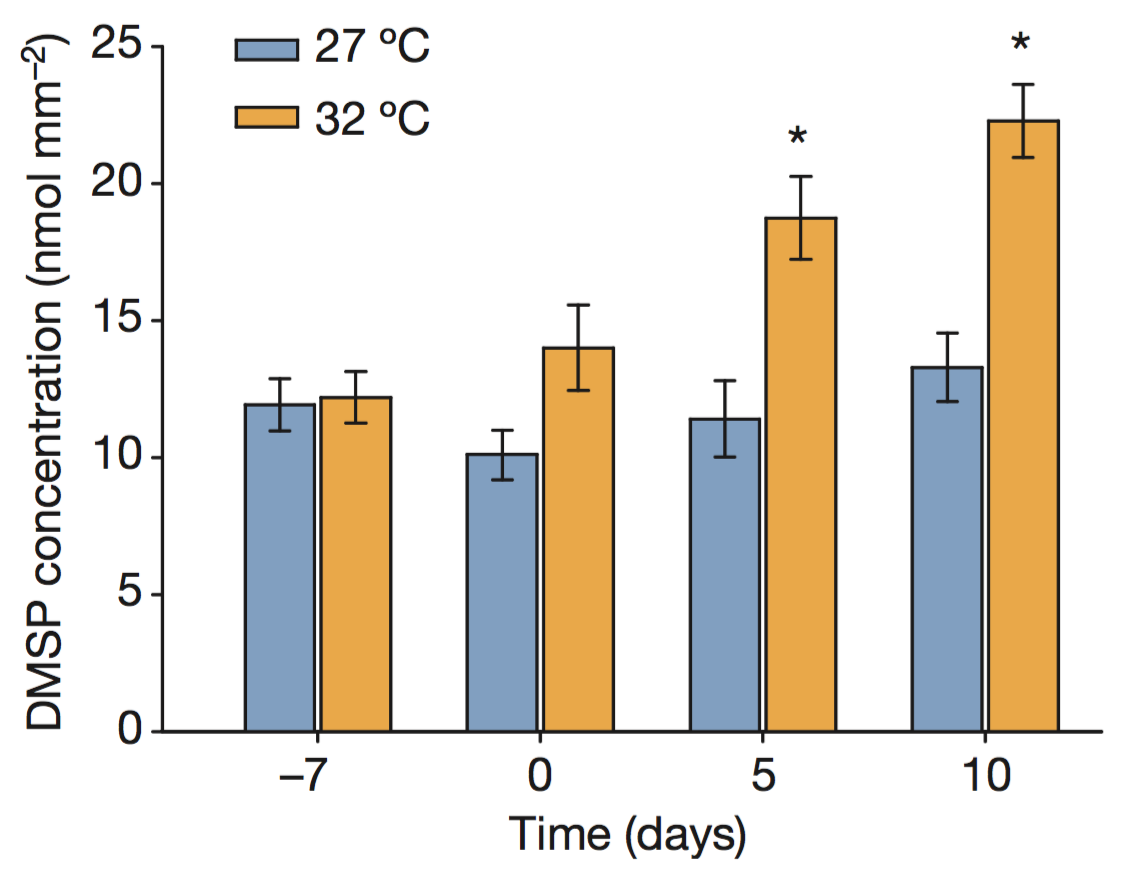
\includegraphics[width=0.7\textwidth,natwidth=1122,natheight=888]{Fig/coraldmspconcvstemp.png}
	    \caption{Adult coral \gls{dmsp} production increases when stressed by a higher temperature over an extended time period \citep{raina:2013fj}.}
	    \label{fig:coralstressdms}
	\end{figure}

	If \gls{dmsp} concentration has a resulting effect on cloud formation through \gls{ccn}, changing coral cover due to changing climate may impact local climate regulation.

	% As the original version of the \gls{claw} hypothesis did not include coral as a producer of \gls{dms}, coral's ability to influence climate was not considered. The temperature and stress dependance of coral \gls{dms} production satisfies the basic requirements of the production mechanism needed for \gls{claw}, but with a constant presence, unlike the blooms of phytoplankton species \cite{Charlson:1987fw}. 


%------------------------------------------------------------------------------------------------------------------
%------------------------------------------------------------------------------------------------------------------

 \section{GBR DMS Production}
 \label{sec:gbrdms}

 	Coral's eventual production of \gls{dms} in the \gls{gbr} region has been explored experimentally. Results from the \gls{gbr} indicate that corals can produce very high concentrations of \gls{dms} and \gls{dmsp} \citep{broadbent2004dms}. These concentrations also appear to depend on \gls{sst}s, and on tidal levels \citep{jones2007factors}. The extent of the \gls{gbr} presents a large source of sulphur that enters the atmosphere \citep{jones:2005ez}. 

 	The \gls{gbr} region is exposed regularly to south-easterly and southerly trade winds, providing the wind shear required to transfer \gls{dms} from the ocean to the atmosphere \citep{liss:1983iu}. During a voyage in $1997$, \citet{jones:2005ez} measured the highest levels of atmospheric \gls{dms} when these trade winds passed over large areas of the reef experiencing low tides (see \cref{fig:dmslowtide}). 

	\begin{figure}[!htb]
	 	\centering
	    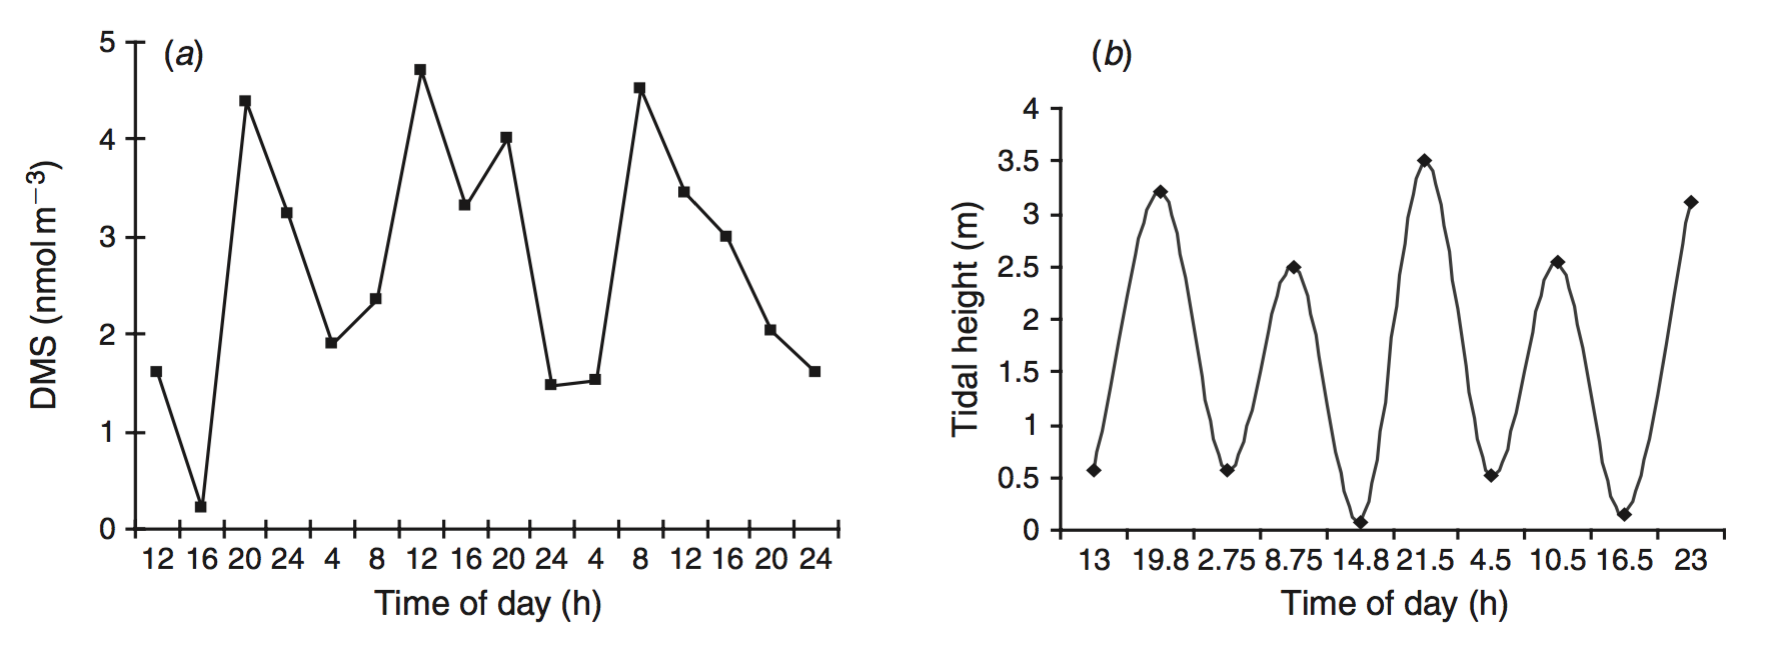
\includegraphics[width=0.9\textwidth,natwidth=1782,natheight=664]{Fig/DMS_tidal_link.png}
	    \caption{Data indicating the presence of a delayed link between atmospheric \gls{dms} concentrations and low tide events in the northern \gls{gbr} and NW Coral Sea \citep{jones:2005ez}.}
	    \label{fig:dmslowtide}
	\end{figure}

 	From here the production of \gls{ccn} from \gls{gbr} sourced \gls{dms} is not as well established. Much depends on the meteorology of the region and the relative concentrations of competing \gls{ccn} and \gls{dms} sinks. Localised modelling is needed to provide predictions in this area of research \citep{cainey:2007jj}.

 	


%!TEX root = Literature_Review_David_Burns.tex
\chapter{Modelling}
\label{ch:model}

Given the nebulous problems in atmospheric science, the best way of obtaining a theoretical description of the systems is through modelling. Generally, a number of models are chained together to simulate different parts of the climate system. Each of these models is built upon a number of theories that are used depending on the state of the system at the time \citep[Chapter 21]{jacobson2005fundamentals}. This makes atmospheric modelling difficult and broad. Fortunately many models have been developed around the world to fill various niches \citep{draxler:1997tga, mann:2010wb, cope:2009tz, mcgregor2008updated}.

The first choice to make when deciding which model to use is between a Global Climate Model (\gls{gcm}) and a Regional Climate Model (\gls{rcm}). The difference is in the granularity achieved in the discretisation used to solve the governing equations, and the requirements of boundary conditions \citep{thatcher:2015wy}. A \gls{rcm} is run on a smaller scale for a specific region with a high density of grid points. As only a small portion of the Earth's surface is simulated, the values of parameters at the boundary of that region must be known in advance \citep{hurley2002air}. Usually these boundary conditions are obtained from a previous run of a \gls{gcm}. Although a \gls{gcm} is less restrictive than a \gls{rcm}, its lack of high resolution may miss small but critical details. Conversely, the regional restriction of a \gls{rcm} can miss distant events that may influence the climate in the simulated region \citep[Chapter 25]{seinfeld2012atmospheric}.

% 'one short paragraph on this'
% What are the base equations most models use?
% Reduced versions of the navier stokes eqns...
% What ways can we numerically solve these equations?
% finite difference
% finite element
% operator splitting
% finite volume?
% 'include a sentence from this in the above paragraph to illustrate approximations'
% Obviously the full blown navier stokes equations are far too complicated to solve. So what approximations are generally used by climate modellers to still encapsulate some of the more complicated flow dynamics?
% An example is eddy diffusivity. Eddy currents occur on both small and large scales and are the result of turbulent flow around obstacles such as land masses 'cite'. A constant called the eddy diffusivity attempts to cover mixing due to eddy currents. I think this is a good example of the limitations in atmospheric models and attempts to use simple equations to approximate more complex phenomena.
% Actually it seems like most models neglect normal diffusion in favour of turbulent diffusion as the rate of turbulent diffusion dominates regular diffusion \citep[Chapter 17]{seinfeld2012atmospheric}.


% Whats the difference between eulerian and lagrangian modelling?
% What is semi-lagrangian modelling? benefits?


% what is sensitivity to initial conditons and what effect does this have on models?
% How can we tell when models are accurate?
% What methods should we use to decide if the model is good? (this is before data is taken so i mean things like sensitivity analysis), cite examples of things like sensitivity analysis, switching various things on and off to understand what is happening.


%--------------------------------------------------------------------------------------------------------------------------%
%--------------------------------------------------------------------------------------------------------------------------%

	\section{Back Trajectory Modelling}
	\label{sec:backtraj}

	When working in atmospheric science, it is often necessary to produce an idea of where a particular parcel of air has travelled from. With the advent of large scale meteorological measurements, the data required to model this process is now being produced. Trajectory modelling is able to take a particular location and predict, forward or backward in time, the path a parcel of air has taken to get there. It can be used to predict whether air at a particular location has passed over a region or event of interest or, for example, whether there has been contamination from anthropogenic sources \citep{draxler:1998vr}.

	\gls{hysplit} is the Hybrid Single Particle Lagrangian Integrated Trajectory model developed by the National Oceanic and Atmospheric Administration and Australia's Bureau of Meteorology. It takes as input a variety of different meteorological data sources to produce the field the parcel travels through. \gls{hysplit}'s efficacy in performing back trajectory modelling is well established \citep{draxler:1998vr}. It has been used to model many different scenarios from forecasting fire smoke movement \citep{rolph:2010in} to nuclear cloud dispersion \citep{rolph:2014kk}.

	A Lagrangian model may be implemented in two different ways. A puff model regularly releases and follows a parcel of air containing the required fraction of trace components. The puff moves and expands depending on advection and diffusion respectively. A particle model releases many single particles which are moved through advection, but which are also randomly moved based on the diffusion present \citep{draxler:1997tga}. \gls{hysplit} implements a hybridisation of these models by using the particle style for vertical motion, and the puff style for horizontal motion \citep{hurley:1994df}.

	%The user provides a location and time for the start of the trajectory, and the amount of time backwards or forwards for it to run. \gls{hysplit} produces a line of lattitude and longitude points where each point is an amount of time away from the starting time. Thus the line through the points indicates the trajectory, backwards or forwards through time of the air at the starting location. 'is this too much like the first paragraph?'

	\gls{hysplit}, like all atmospheric models, is sensitive to initial conditions \citep{challa2008sensitivity} and its accuracy is dependent on the error margins of the meteorological data it makes use of \citep{draxler:1998vr}. The results of any trajectory run are therefore less accurate the further away from the initial conditions the trajectory gets. There is also a dependence on the spatial and temporal granularity of the meteorological data. As such, \gls{hysplit} offers the ability to slightly permute the initial conditions of the model to produce a multitude of possible trajectories for a single location and time \citep{draxler:1997tga}. It is also possible to produce multiple trajectories over time or over space and a robust scripting platform exists to allow this \citep{draxler:1997tga}.

	% I think we should keep this for the section where we actually do work...

	% \subsection{\gls{hysplit} Visualisations}
	% \label{subsec:hysvis}

	% 	A technique for producing meaningful visualisations of this modelling system, given it's shortcomings, is to produce a probability density function of multiple potential trajectories. The GUI side of \gls{hysplit} offers a method for doing this using the bulk production of trajectories from permuted initial conditions \citep{draxler:1997tga}.  A spatial domain is subdivided into boxes, then whatever points of the various trajectories that lie in that box are counted. Each box is then normalised by the total number of trajectory points in the domain. It is then possible to plot these boxes onto a map of the region, colouring them based on their values. This technique provides a visual idea of the probability that a given parcel of air will have passed over that box. Similarly, by producing multiple trajectories over time, it is possible to create a visualisation of the probability a parcel of air has passed through a box within a time period. 'should i put an example here?'
	% 	'should i talk about plotting the exact trajs and then animating it over time?'
	% 	If the number of points in box $i$ is $N_i$ then the probability of the parcel of air being in that box $p_i$ is given by,
	% 	\begin{align}
	% 		p_i = \frac{N_i}{\sum_{i=1}^m N_i},
	% 	\end{align}
	% 	where $m$ is the total number of boxes \cite[Chapter 3]{Lefebvre:2006vi}.

	% 	Another visualisation tool is to create a time series of the trajectories, overlaid on a map, in a movie. This shows how the trajectory evolves with the changing meteorological conditions. This could be coupled with \gls{pdf}s computed using small variations of the initial conditions to produce a better idea of probable trajectories' evolution through time.




%--------------------------------------------------------------------------------------------------------------------------%
%--------------------------------------------------------------------------------------------------------------------------%

	% \section{Unified Model}
	% \label{sec:unimod}
	% 'contemplate dumping this paragraph'

	% The Unified Model (\gls{um}) is a suite of models produced by the United Kingdom Met Office. One of the submodels for dealing with chemistry and aerosols is the United Kingdom Chemistry \& Aerosols model \gls{ukca}. One of the aerosol sub models for \gls{ukca} is \gls{glomapm}. This is a version of a combined meteorological, chemical, and aerosol model with feedback throughout the submodels 'site some unified model description paper'.

%--------------------------------------------------------------------------------------------------------------------------%
%--------------------------------------------------------------------------------------------------------------------------%

	\section{CCAM, CTM, GLOMAP}
	\label{sec:ccg}

	The three models to be used in this project are \gls{ccam}, \gls{ctm} and \gls{glomapm}. \gls{ccam} provides the meteorological data needed for \gls{ctm} and \gls{ctm} provides the chemical concentration data required for \gls{glomapm}. However, currently the system is limited to running \gls{ccam} offline from the other models (see \cref{fig:modelstruct}) \citep{mcgregor2008updated}. Thus there is no feedback into the meteorology from changes in aerosol levels, such as cloud production caused by changes in \gls{ccn} concentrations.

	\begin{figure}[!htb]
	    \centering
	    \vspace*{5mm}
	    \includegraphics[width=0.8\textwidth]{Fig/ModelStructure.tikz}
	    \vspace*{5mm}
	    \caption{The group of models prepared by \gls{csiro} for modelling from meteorology to aerosols. Arrows indicate the direction data passes.}
	    \label{fig:modelstruct}
	\end{figure}

	This combination of models has been used previously in the Sydney Particle Study \citep{cope:2014tw}. The Sydney Particle Study was a large scale study performed by seven different organisations and lead by CSIRO. It encompassed both measurement and modelling of fine particles in the Sydney area, with a view to understand their exposure to Sydney's population. Both \gls{ccam} and \gls{tapm} (an alternative meteorological model produced by \gls{csiro}) were used as the \gls{rcm}s for the study. Their outputs were compared with each other, and with the collected data. \gls{ctm}, and consequently \gls{glomapm}, were used for the particle dynamics and chemical transport modelling within the two \gls{rcm}s. Both \gls{rcm}s performed well, with predictions of sea salt, organic matter and secondary inorganic aerosols within \SI{15}{\percent} of observations (see \cref{fig:sydpartdata}) \citep{cope:2014tw}.

	\begin{figure}[!htb]
	    \centering
	    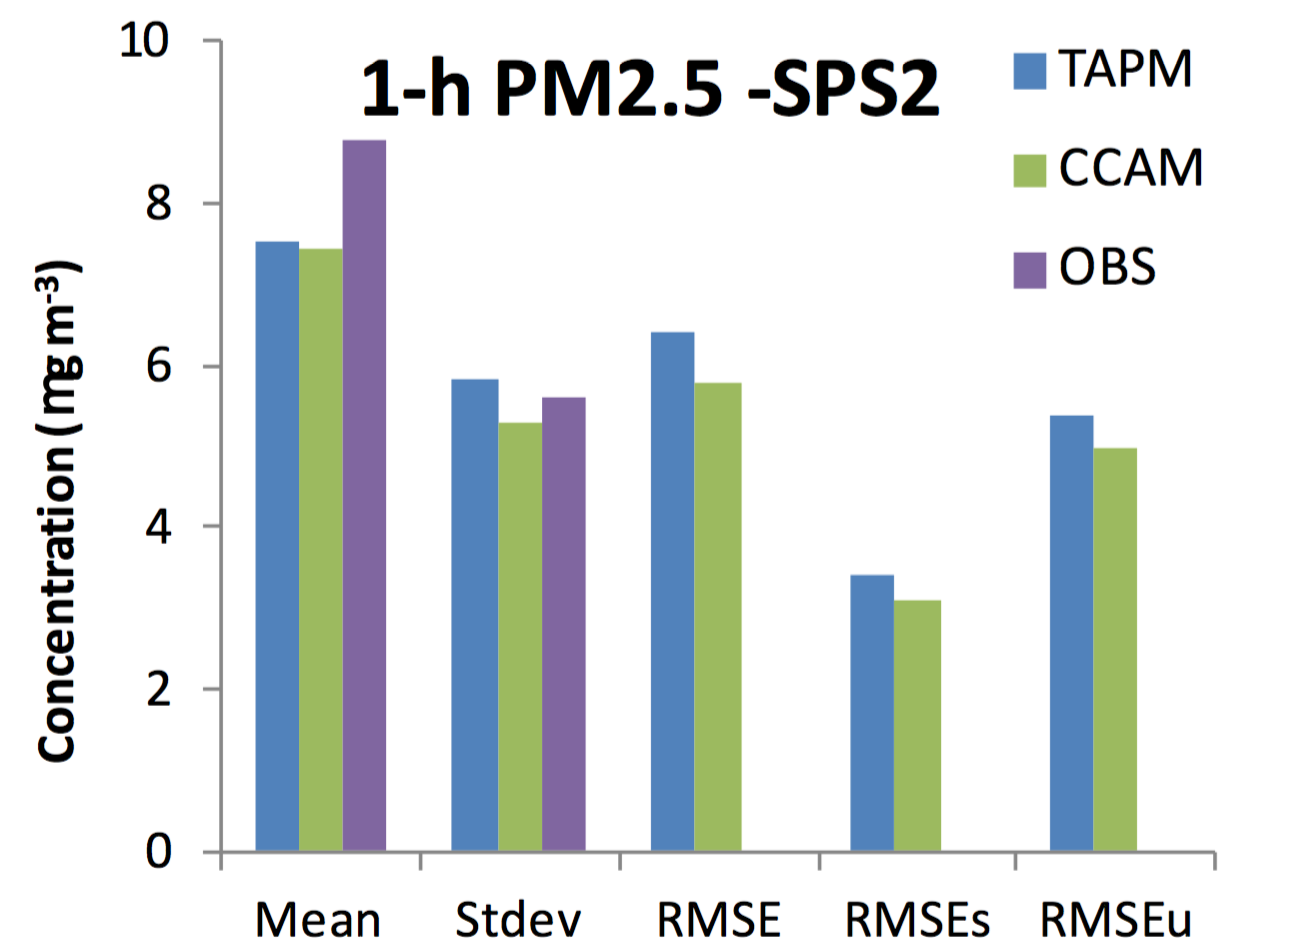
\includegraphics[width=0.6\textwidth,natwidth=1308,natheight=952]{Fig/sydneyparticledata.png}
	    \caption{The hourly averaged concentrations of PM2.5 particles for the second Sydney Particle Study. Both \gls{ccam} and \gls{tapm} used as the base meteorological model produce similar average concentrations, close to observation \citep{cope:2014tw}.}
	    \label{fig:sydpartdata}
	\end{figure}




%--------------------------------------------------------------------------------------------------------------------------%

		\subsection{CCAM}
		\label{subsec:ccam}

		\gls{ccam} is \gls{csiro}'s Conformal-Cubic Atmospheric Model. Most \gls{rcm}s are performed on a grid that simulates only the area of interest, requiring spatial boundary conditions to be fed into the model at each time step \citep{hurley2002air}. Because of \gls{ccam}'s approach of conformal cubic mapping, the majority of grid points can be focussed onto the region of interest while still simulating the rest of the globe with a gradient of accuracy (see \cref{fig:ccammap}). This removes the necessity for boundary conditions as the full globe is being simulated. This allows distant events to influence the region of interest. However, there are fewer grid points in distant regions, sacrificing accuracy for computation time \citep{mcgregor:2005wz}.

		\begin{figure}[!htb]
	    	\centering	    

  			\begin{subfigure}[b]{0.8\textwidth}
  				\centering
	    		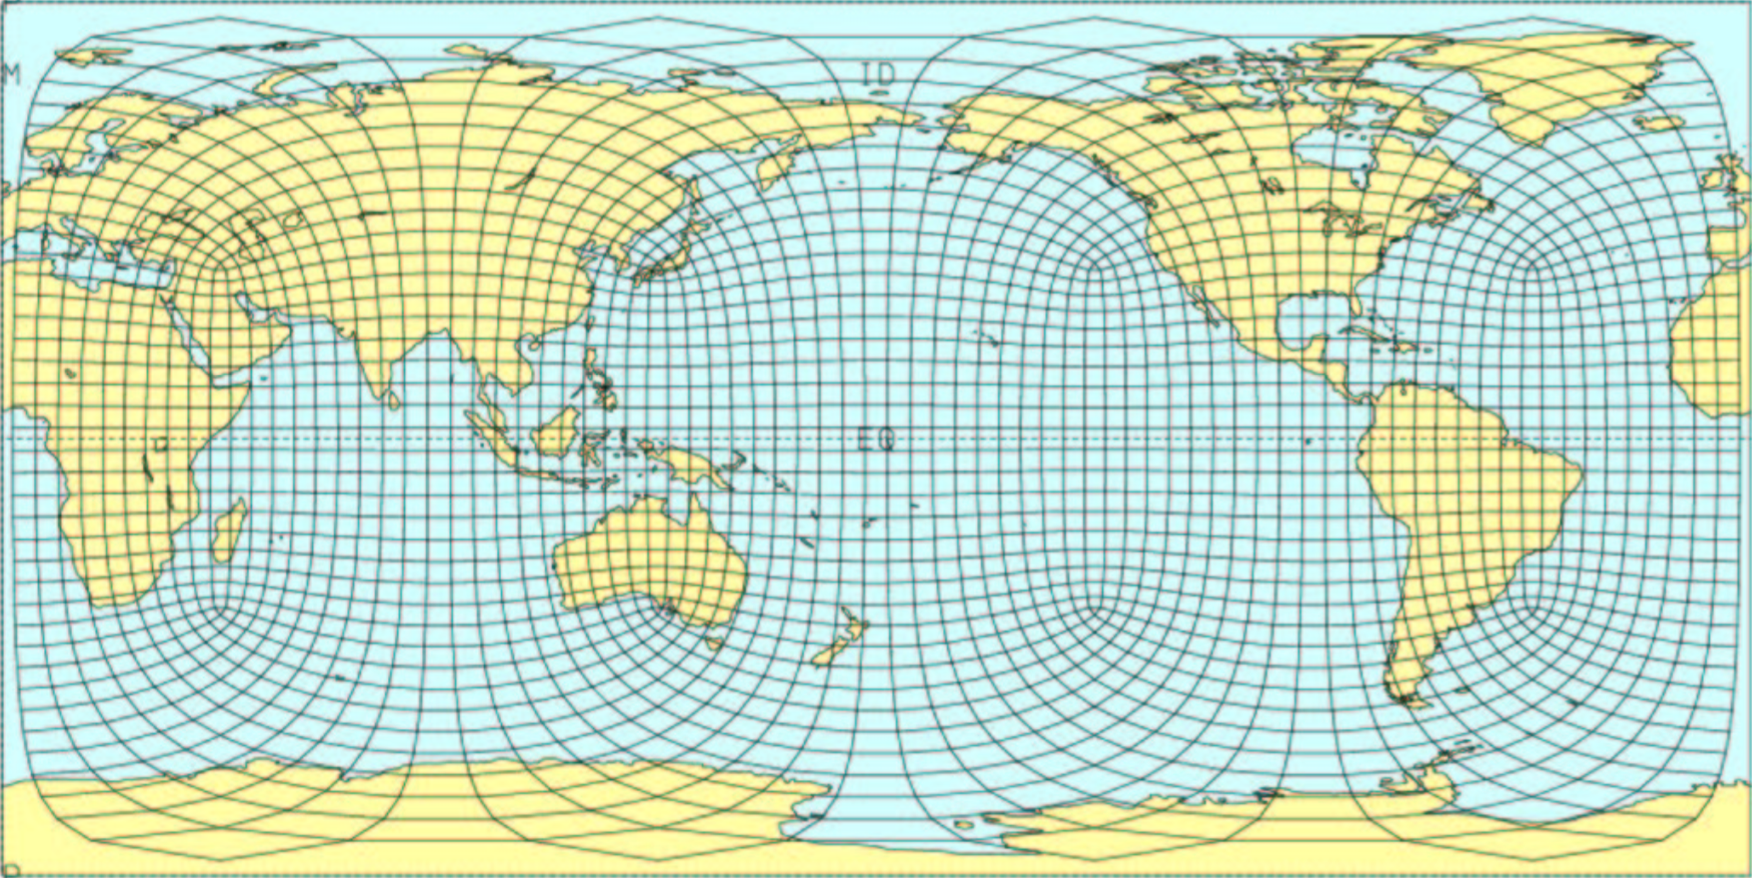
\includegraphics[width=\textwidth,natwidth=1752,natheight=878]{Fig/ccamnormal.png}
   				\caption{}
   				\label{fig:ccammapnorm} 
			\end{subfigure}

			\begin{subfigure}[b]{0.8\textwidth}
			\centering
	    		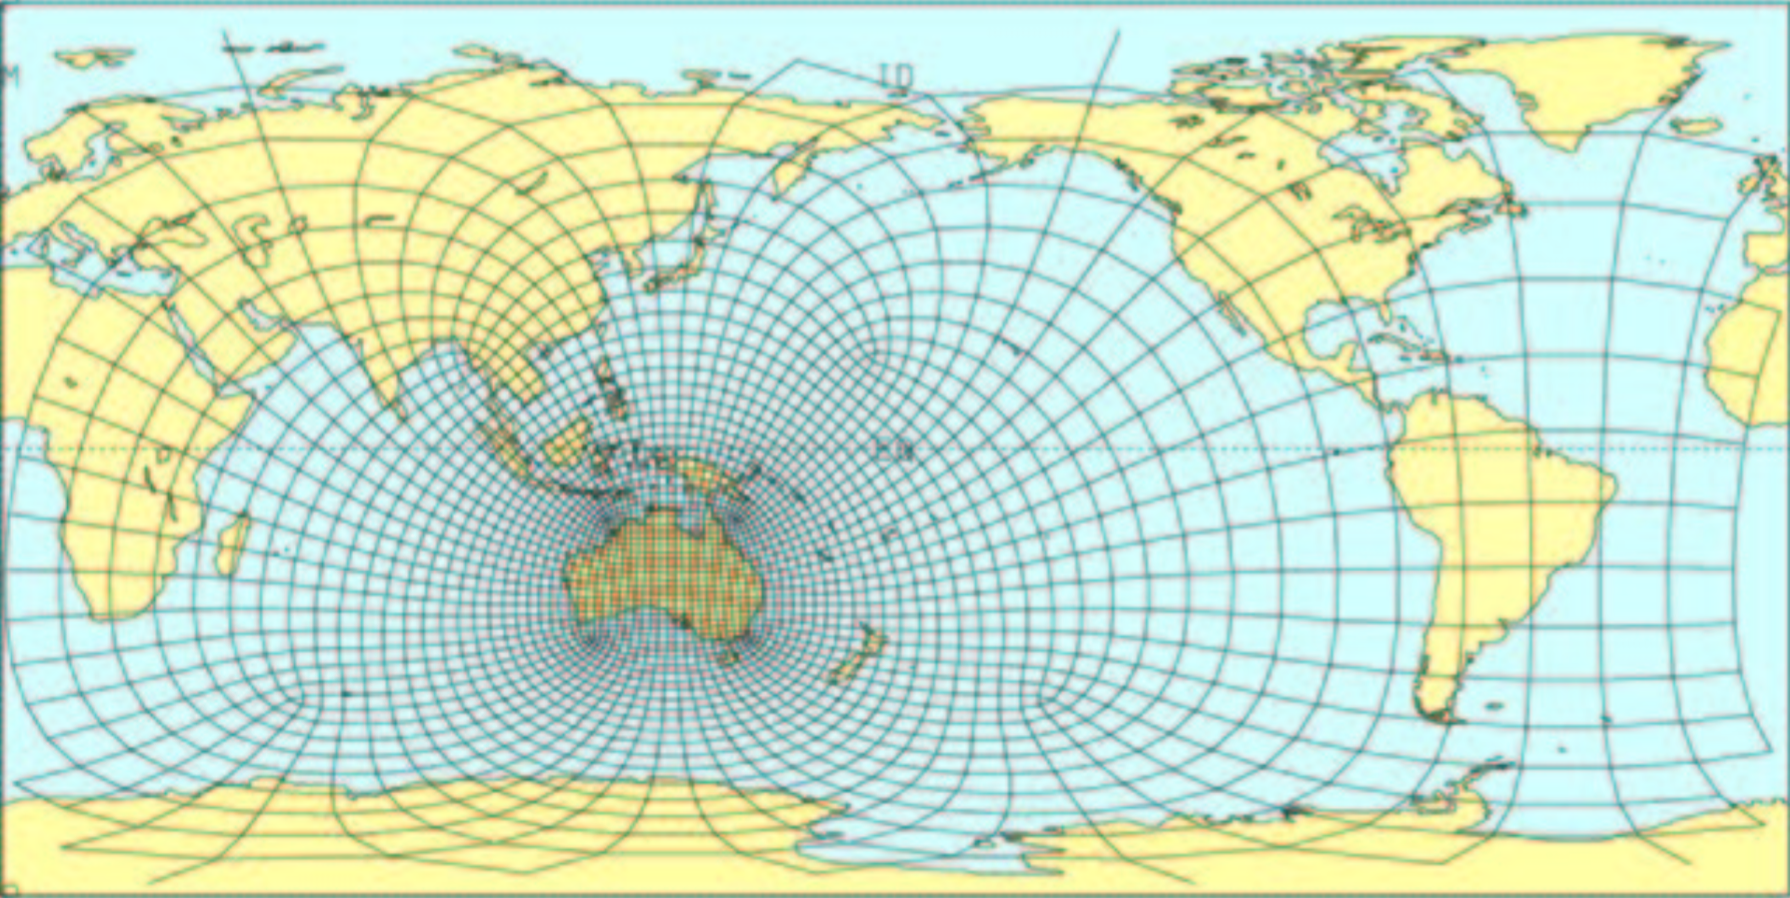
\includegraphics[width=\textwidth,natwidth=1790,natheight=898]{Fig/ccamfocussed.png}
				\caption{}
				\label{fig:ccammapfocus}
			\end{subfigure}

			\caption{Two examples of the conformal cubic mapping, used by \gls{ccam}, showing both a focussed and unfocussed transformation of the grid \citep{mcgregor:2005wz}.}
	    	\label{fig:ccammap}
		\end{figure}

		%The cubic grid structure creates a number of numerical problems. The most obvious is the existence of singularities at the corners. 'I think ccams semi-lagrangian approach helps here, and some paramters are treated differently... this is all in the ccam description papers but i dont understand it yet'

		As inputs \gls{ccam} can accept data sets from a \gls{gcm} and nudge the model towards these values \citep{mcgregor:2005wz}. Although work is being done to incorporate a coupled ocean model with matching grid structures, without this the oceanic parameters, such as sea surface temperature, must be input as both spatially and temporally varying maps \citep{mcgregor2008updated}. Despite the non-uniformity of the cubic grid structure, \gls{ccam} produces latitude and longitude based output through interpolation of the cubic grid data \citep{thatcher:2015wy}.

		The current implementation of \gls{ccam} uses a semi-Lagrangian solver that is semi-implicit and non-hydrostatic, programmed in FORTAN. The solver is designed for expansion to a large number of cores, while dealing with the singularity-like points caused by the cubic mapping \citep{thatcher:2015wy}. It is also possible to run the model multiple times, focussing the grid in at each step while nudging is performed using the previous runs' data \citep{mcgregor2008updated}.


%--------------------------------------------------------------------------------------------------------------------------%

		\subsection{CTM}
		\label{subsec:ctm}

		\gls{ctm} is the Chemical Transport Model produced at \gls{csiro}. It deals with various transport processes relating to chemicals found in the atmosphere, as well as deposition onto particles, changes in chemical structure, and emission sources \citep{cope:2009tz}. It uses a regular grid structure which requires boundary conditions (see \cref{fig:sydpartgrid}) that are usually taken from a \gls{gcm} \citep{cope:2014tw}. The transport of each chemical species is modelled using an advection diffusion equation around the chemical's concentration, with source terms relating to different chemical processes. Each of these are themselves modelled and solved before being fed back into the advection diffusion solver \citep{cope:2009tz}. 

		\begin{figure}[!htb]
	    	\centering
	    	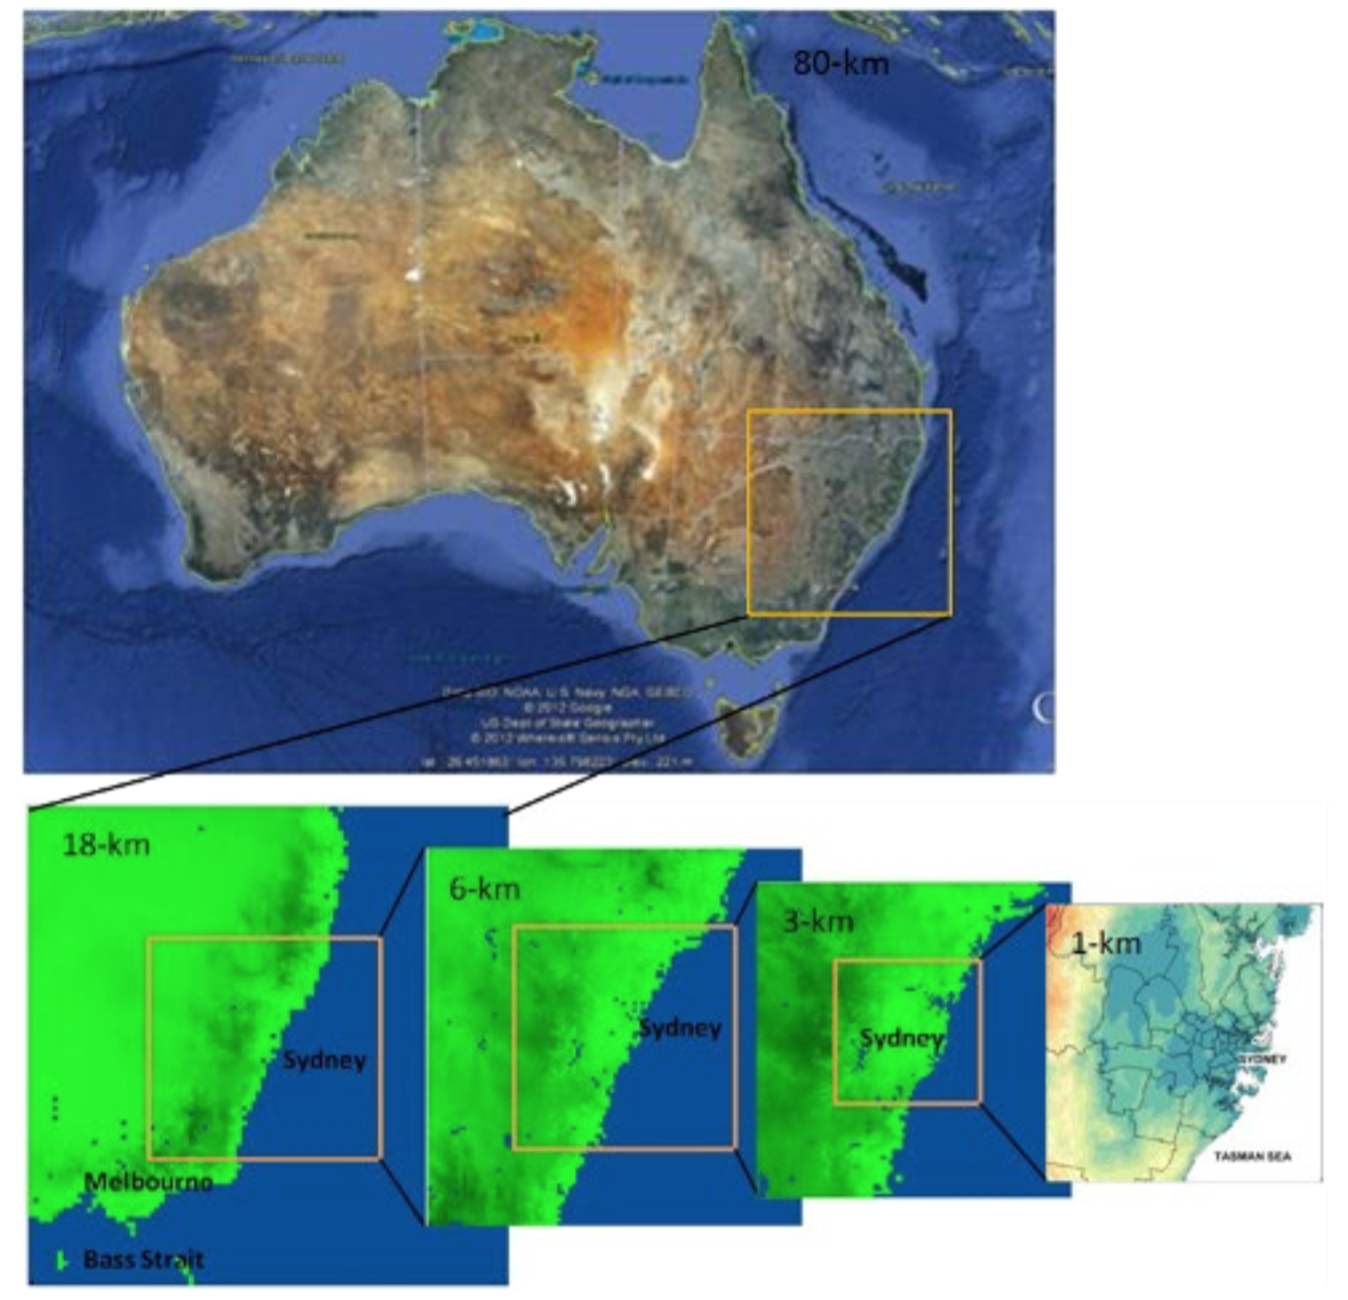
\includegraphics[width=0.8\textwidth,natwidth=1308,natheight=952]{Fig/ctmexample.png}
	    	\caption{A series of the zooming \gls{ctm} grids used in the Sydney Particle Study. An example of a \gls{ctm} produced chemical concentration map can be see at the bottom right \citep{cope:2014tw}.}
	    	\label{fig:sydpartgrid}
		\end{figure}

		\gls{ctm} is also written in FORTRAN, but allows for chemical reactions to be entered as regular form chemical equations \citep{cope:2009tz}. It requires a meteorological map as input, along with initial and boundary conditions for each chemical being tracked. Maps for the introduction of chemicals from the surface to the atmosphere are also required, such as when \gls{dms} is produced by the \gls{gbr}. \gls{ctm} outputs atmospheric maps of chemical concentrations.

%--------------------------------------------------------------------------------------------------------------------------%

		\subsection{GLOMAP and GLOMAP-mode}
		\label{subsec:glomap}

		\gls{glomap} is the aerosol micro-physics component of the \gls{ukca} model developed at Leads university. It uses atmospheric information and chemical concentrations to simulate the large amount of interactions aerosols undergo. It models new particle formation, condensation, cloud processing, hygroscopic growth and many other aerosol processes \citep{mann:2010wb}.

		\gls{glomapm} is an alternate version of \gls{glomap} which segregates aerosols via modes (see \cref{sec:aerosols}) rather than the \gls{glomap}'s direct bin approach. \gls{glomapm} also uses the equilibrium Henry's law style aqueous phase reactions recommended by \citet{barnes:2006ug}, while \gls{glomap} uses a more computationally expensive diffusion limited method \citep{mann:2010wb}. Both differences make \gls{glomapm} less accurate, but also less computationally expensive. Some treatments of particles are also adjusted to better make use of the modal structure. An example is that \gls{glomap} applies rain-out to any particles over \SI{103}{\nm}, while \gls{glomapm} applies rain-out to soluble particles in the accumulation and coarse modes \citep{mann:2010wb}. For modelling \gls{dms} and its aerosol products, \gls{glomap} uses the sulphur oxidation steps outlined in \citet{seinfeld2012atmospheric} and precomputed Henry's law coefficients \citep{mann:2010wb}. 

%'There is a whole section in \citep{Mann:2010wb} that describes the nucleation of new sulfate aerosol. Perhaps you should do an analysis of it comparing its treatment to current research? God this could be a whole section in and of itself... There are a bunch of good references in this section which you can take a look at.'
%Is this method adequate based on the stuff we have already talked about in regard to the sulfur cycle?
% this section might need a boost from "Impact of nucleation on global CCN"

		The chemical concentration maps needed to feed into \gls{glomap} can either be offline, computed beforehand, or online \citep{mann:2010wb}. Online maps are updated by what is consumed or produced within \gls{glomap} and then passed to a chemical transport model running above \gls{glomap} \citep{spracklen2003development}. \gls{glomap} produces maps of aerosol concentrations, separated into bins or modes depending on the version used.

		%there is no aitken mode sea salt produced by the model... from luke



%!TEX root = Literature_Review_David_Burns.tex
%ergh maybe just cut the shit out of this, we are just going to focus on a simple constant release anyway to start

\chapter{DMS Climatology Modelling}
\label{ch:dmsclim}

The way in which \gls{dms} is created and enters the atmosphere needs to be considered when attempting to model its effects on climate. There are a number of ways in which this can be treated: using large data maps, modelling the ocean, and/or applying different methods for ocean surface to atmosphere exchange (surface flux) \citep{woodhouse:2010ed}. These climatological models of \gls{dms} are needed to produce the chemical concentration maps used as input for any chemical transport model (see \cref{subsec:ctm}).

	\section{Modelling DMS production}
	\label{sec:modeldms}

	A number of studies exist for modelling \gls{dms}. Their methods provide guidance for which modelling systems are successful, and which \gls{dms} climatological models are necessary to produce realistic results.

	The Pacific Atmospheric Sulfur Experiment (\gls{pase}) measured \gls{dms} and \gls{sot} levels via flights made at \SI{40}{\metre} above sea level in the remote Pacific Ocean, near Christmas Island \citep{bandy2011pacific}. Other chemicals were also measured, including \gls{h2so4}. Using this data \citet{simpson:2014} devised budgets for \gls{dms}, \gls{sot} and \gls{nss} sulphate particles. The \gls{dms} budget consisted of surface flux, entrainment, oxidation and divergence. Using the budgets it was calculated that approximately \SI{20}{\percent} of \gls{dms} became \gls{nss} sulphate particles. 

	In the region measurements were taken from, an easterly jet stream from South America introduced \gls{nss} sulphate particles, originating from the land, into the \gls{mbl}. This was exacerbated by a localised subsidence. Modelling showed that the particles introduced via \gls{ft} entrainment dominated those produced from \gls{dms} for the region \citep{simpson:2014}. The study revealed that their results were influenced by regionally specific inputs that may not be present in the \gls{gbr}, and highlights the importance of localised modelling and the potential influence of particles from the \gls{ft} \citep{simpson:2014}.

	\citet{woodhouse:2010ed} produced a global model of \gls{dms} and its effects on \gls{ccn} concentration. Aerosol processes were modelled using \gls{glomapm} inside of a chemical transport model called TOMCAT. A number of \gls{dms} climatologies were tested, with the climatology developed by \citet{Kettle:2000jy} as a reference point (see \cref{sec:dmssurf}). The model showed that \gls{dms}'s highest impact on \gls{ccn} was in the southern hemisphere (see \cref{fig:wooddmsccn}). Also, any region with large anthropogenic \gls{ccn} sources sees little impact from \gls{dms} \citep{woodhouse:2010ed}. Overall, the global impact of \gls{dms} on \gls{ccn} in the model was low. It was also found that changes to \gls{ccn} production from different climate change scenarios could not be distinguished from variances arising from using different climatology models.

	\begin{figure}[!htb]
	    \centering
	    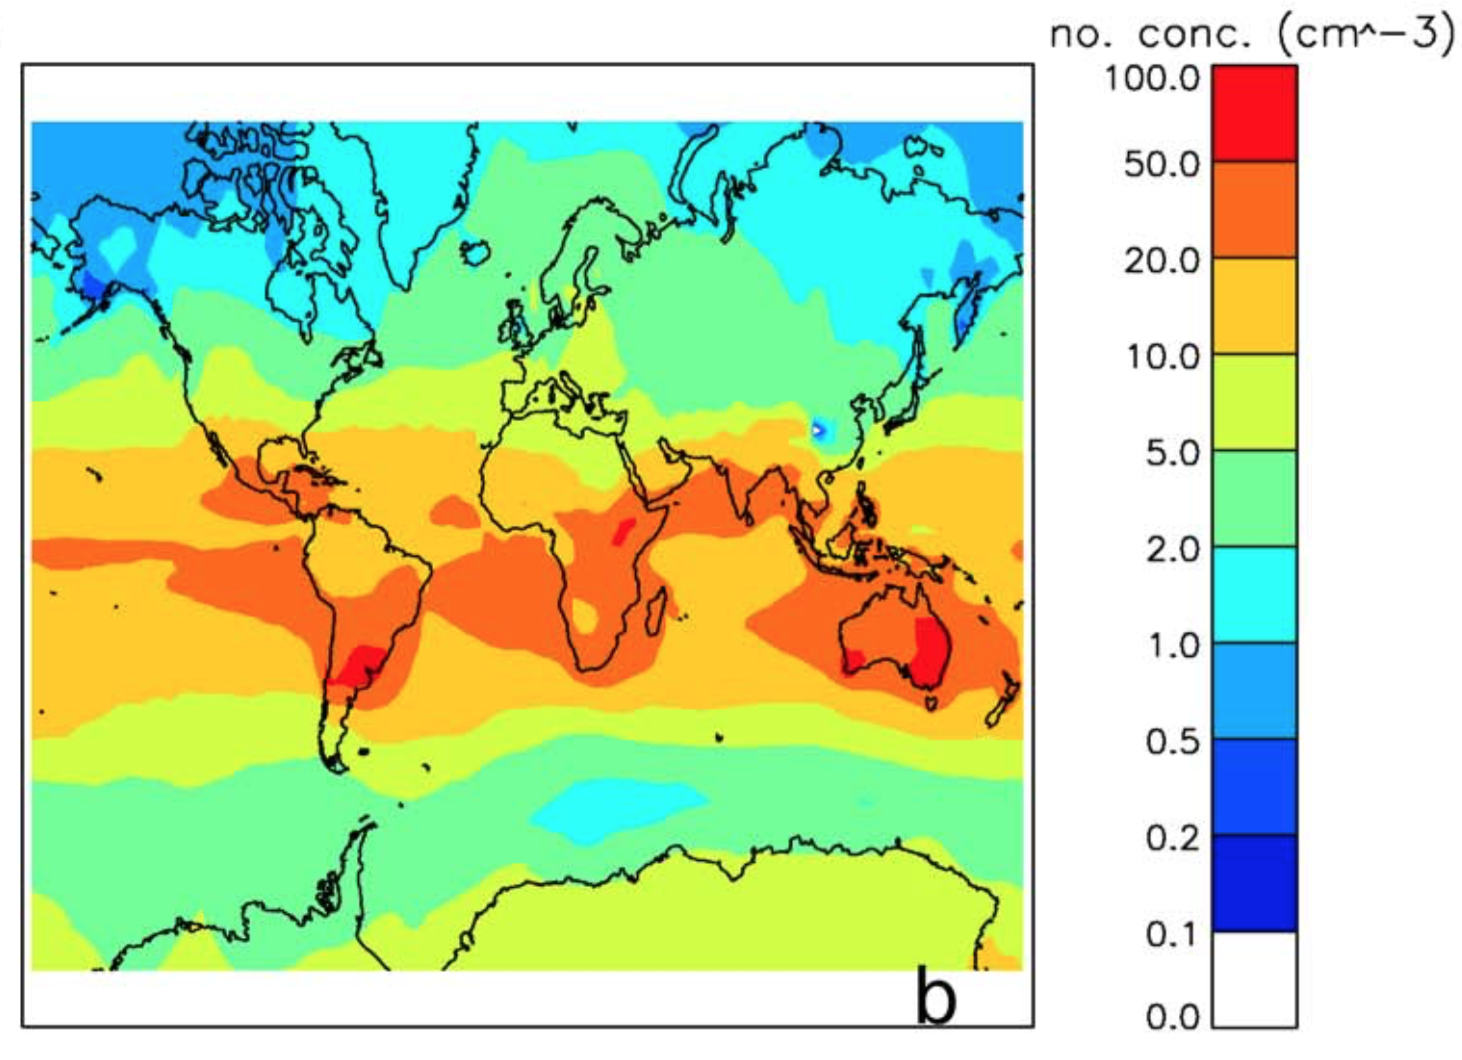
\includegraphics[width=0.6\textwidth,natwidth=1462,natheight=1060]{Fig/wooddmsccn.png}
	    \caption{A global map of the difference between \gls{ccn} concentrations produced by model runs with and without \gls{dms} \citep{woodhouse:2010ed}.}
	    \label{fig:wooddmsccn}
	\end{figure}

	% What has been done around modelling in the southern hemisphere and the \gls{gbr} region specifically? Does this level of regionality matter in terms of modelling these processes?


%--------------------------------------------------------------------------------------------------------------------------%
%--------------------------------------------------------------------------------------------------------------------------%

	\section{DMS Surface Flux}
	\label{sec:dmssurf}

	As mentioned in \cref{subsec:ctm}, maps of the chemicals being analysed are required to feed into any chemical transport model used. For \gls{dms}, this is often given as a surface flux map for the region of interest. There are many meteorological and biological variables influencing \gls{dms} surface flux. The major meteorological variable is wind speed at the surface of the ocean \citep{Kettle:2000jy}. Surface concentrations of \gls{dms} are generally taken from experimental data with a flux model producing atmospheric concentrations \citep{woodhouse:2010ed}.

	\citet{Kettle:2000jy} describes a methodology for approximating a global \gls{dms} surface flux map. Data was collected from a large number of publications, study databases and direct correspondence with researchers (see \cref{fig:kettledata}). The data was then interpolated to provide monthly global \SI{1}{\degree} resolution sea surface \gls{dms} maps. Maps for sea surface salinity, temperature and chlorophyll concentration were also created \citep{kettle1999global}. In \citet{Kettle:2000jy} the surface concentration maps from \citet{kettle1999global} were converted to surface flux maps using a technique from \citet{liss:1983iu} The transfer rate was assumed to be a function of the concentration difference between the ocean and air, and the piston velocity, which depends on wind speed. Other surface flux methods were also examined and the differences between them produced an error in \gls{dms} results greater than \SI{50}{\percent}. Overall, the method showed little dependence on meteorological changes to \gls{dms} flux, around \SI{10}{\percent} for future predicted changes.

	\begin{figure}[!htb]
	    \centering
	    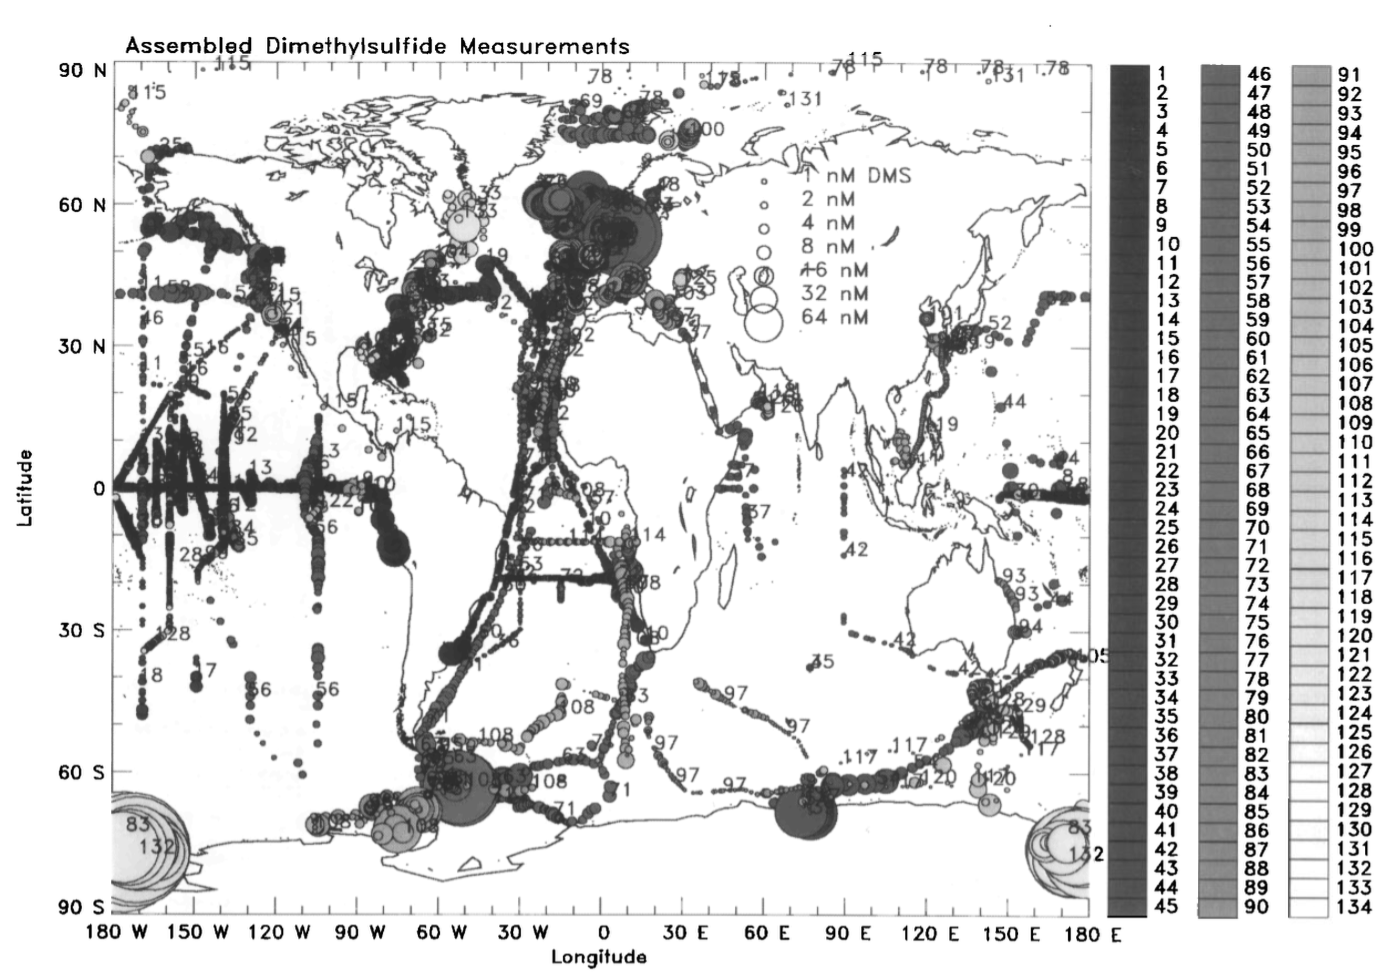
\includegraphics[width=0.8\textwidth,natwidth=1414,natheight=1344]{Fig/kettledata.png}
	    \caption{The global measurement data used for producing interpolated maps of \gls{dms} sea surface concentrations \citep{kettle1999global}. Larger circles indicate higher concentrations while shading defines the contributor.}
	    \label{fig:kettledata}
	\end{figure}

	\citet{lana2011updated} expanded on this work producing a more complete and accurate climatological model of \gls{dms} surface flux. Their model indicates a summer increase in surface flux (see \cref{fig:lanadmsmaps}) and also a vertical dependence on atmospheric \gls{dms} concentration. The database of measurements used was also three times larger than that of \citet{kettle1999global}, resulting from continued efforts into the SOLAS project (Surface Ocean Lower Atmosphere Study) \citep{lana2011updated}.

	\begin{figure}[!htb]
	    \centering
	    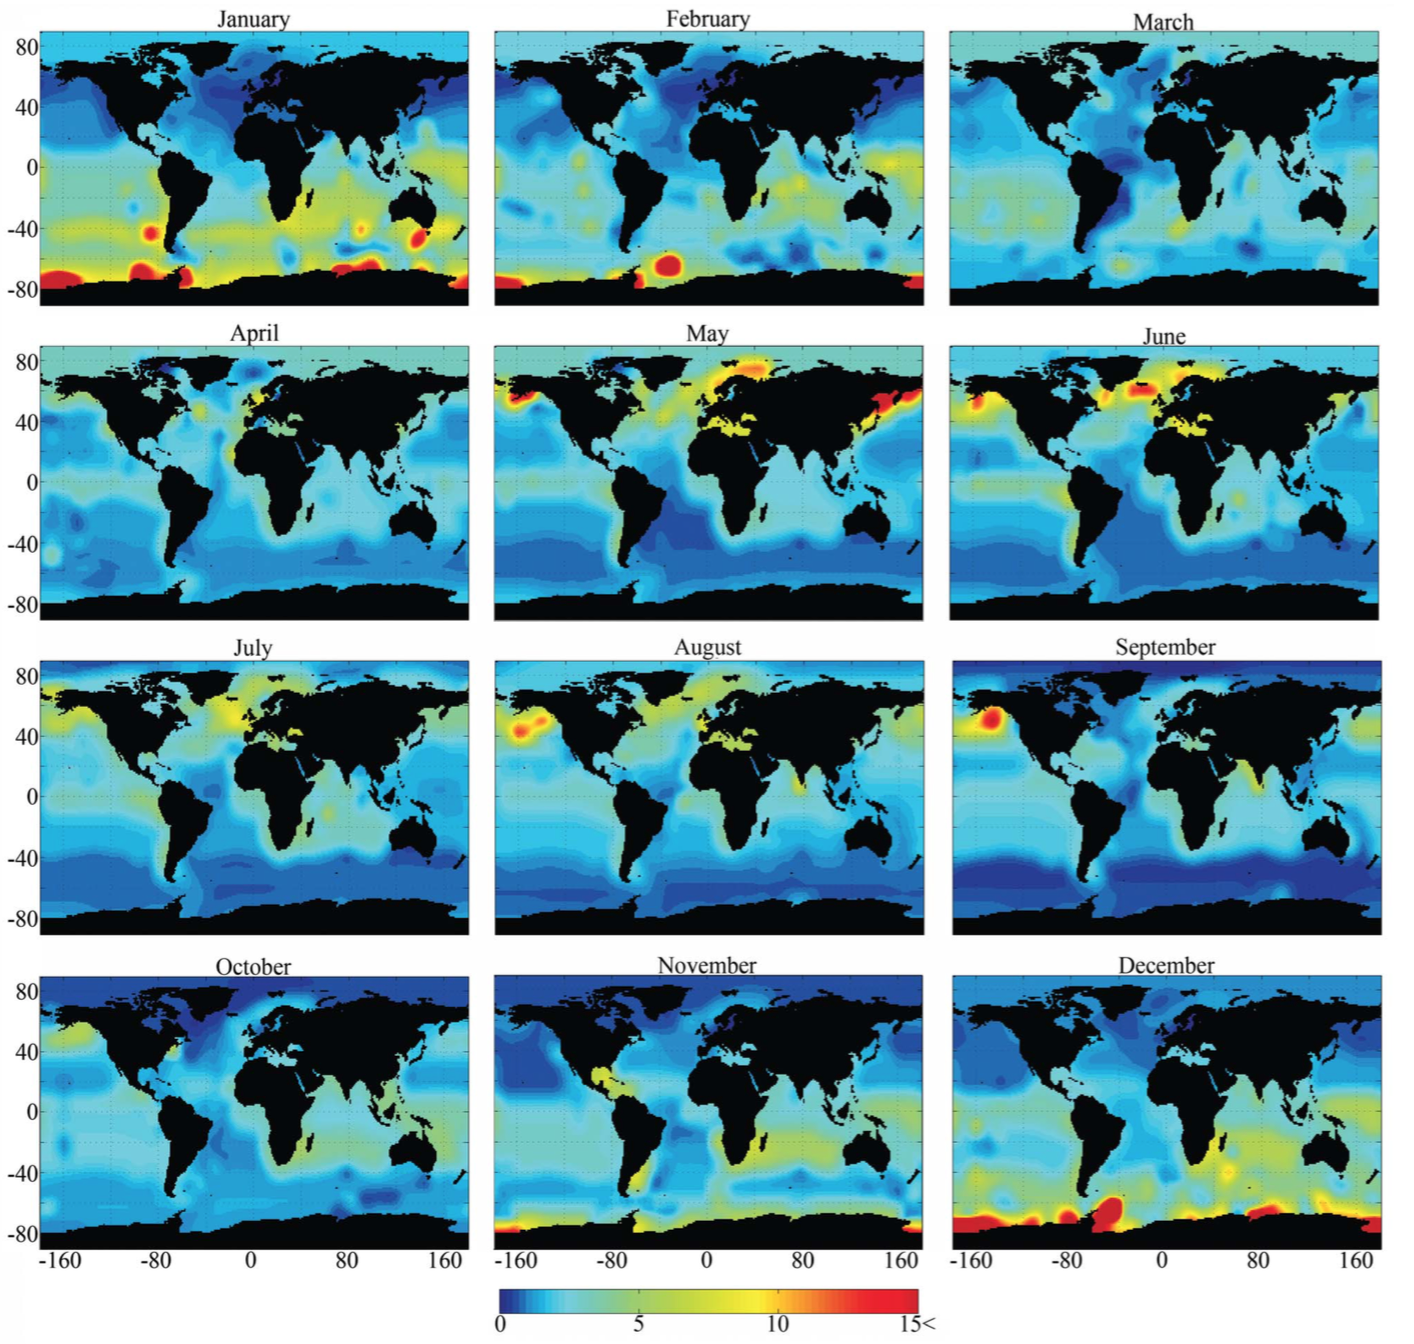
\includegraphics[width=0.9\textwidth,natwidth=1414,natheight=1344]{Fig/lanadmsmaps.png}
	    \caption{Monthly global maps of \gls{dms} concentrations produced using surface concentrations and an updated surface flux parameterisation \citep{lana2011updated}. Increases in \gls{dms} concentrations during summer periods can be seen.}
	    \label{fig:lanadmsmaps}
	\end{figure}

	The observational data for the \gls{gbr} was largely sourced from \citet{jones:2005ez}. Interestingly, both ocean surface and atmospheric \gls{dms} concentrations were measured in this study. The significance of a regional and diurnal dependence on \gls{dms} concentrations indicates that the global results obtained in \citet{lana2011updated} should not be assumed for regionally specific models.



	% What methods are around for estimating the flux?
	% constant, kettle, nightingale, lana
	% kettle describes a large collection of sea surface dms concentrations which is then interpolated to cover the entire globe, 
	% how are these papers tied together? what does each do individually?
	% what are the actual functions that relate sea surface concentraions to atmos concentrations?

	% Is Jones data for the \gls{gbr} used in these inventories? 'some early data was'

	% What effect does changing climate and meteorology have on these fluxes?
	% Globally wind speed is the dominant process.
	% There may be some correlations found in the local \gls{gbr} region that could be used to form some time and met dependent source functions. 'need to explore some of jones papers for this'. This is about the tide link found in jones paper.


	% Has anyone actually made surface concentration measurements at the \gls{gbr}?
	% What does Graham Jones have to say about this? Has he replied to your email?




%--------------------------------------------------------------------------------------------------------------------------%

		% \subsection{Kettle et al.}
		% \label{subsec:kettle}

		% The Kettle paper is a treasure trove of old DMS surface concentration papers. There are hundreds of sources in the introduction and it seems to be really complete. Of course the paper itself is over 15 years old now.

		% Supposedly there is a database available of dms concentrations from geia... I couldn't find it, but maybe it's there. Kettle mentions it.

		% They used a method similar to other well established global emission maps. A large quantity of experimental data was collected from publications and directly from scientists. This included DMS surface concentrations along with a number of other values like ocean height, temperature 'put actual list here'. 

		% The estimates of the error produced in this paper may not encompass errors associated with coral reef production of DMS. They use some strange method for producing the approximated error that I don't understand too well. However they use a comparison with chlorophyll which is not necessarily a good indicator for coral reef produced DMS. Does the coral or it's symbiot even have the type of chlorophyl Kettle uses?

		% There is very little correlation between their DMS map and other maps of various climatological measures. The highest was surface temperature, then chlorophyll a concentration.

		% They have split the world map up into sections, one of which is AUSE, the east coast of Australia. From the figures it appears to be almost constant spatially and temporally. This doesn't seem to match the variability of measurements taken by Jones et al.

		% It might be a good idea to include one of the global map images that is in the Kettle paper. It gives a good idea of what the method actually is. Probably the one on 434.

		% "Smoothed maps must be viewed skeptically because the data assimilation scheme was based mostly on modeled and extrapolated data and should therefore be corroborated with more measurements. Still, the scheme illustrates the kind of fields which could be generated with a larger database of observation." from Kettle. Has there been another attempt at this with newer databases?

		% I don't really get what the big deal is with this paper. It doesn't really provide a usable map. They collected a database of experimental data, mapped it to a globe and then used some smoothing functions. I would need to get the data they used to do anything, and anyway, they haven't really outlined very well the sorts of mathematical techniques they used for their smoothing. They mention a few papers along the way that I should probably look at that are meant to talk about the approximating techniques used.

		% I think perhaps the idea of the paper is that you are meant to get the latest data on DMS measurements and then follow their smoothing and approximation techniques.


%--------------------------------------------------------------------------------------------------------------------------%
%--------------------------------------------------------------------------------------------------------------------------%

	% \section{DMS Surface Flux Paramterisations}

	% what is this about?

	% what different methods are there for defining these parameters?

	% what sort of variability arises from this?

	% talk about the frankly insane levels of varioability from these different methods. What does this mean for any model that makes use of them?

	% nightingale and lana?
	% % 		what are the actual functions that relate sea surface concentraions to atmos concentrations?



% 'i think dump these subsections and keep them to a paragraph explaining the progressions of dms climatological modeling'
%--------------------------------------------------------------------------------------------------------------------------%

% 		'do we need a section here specifically for taking ocean dms concentrations and turning them into atmos concentrations?'
% 		\subsection{Nightingale}

% 		what are the actual functions that relate sea surface concentraions to atmos concentrations?




% %--------------------------------------------------------------------------------------------------------------------------%

% 		\subsection{Lana}




%--------------------------------------------------------------------------------------------------------------------------%
%--------------------------------------------------------------------------------------------------------------------------%

	% \section{Mechanistic Model of DMS surface concentrations}

	% why is this important? what benefits are there over observations?

	% what are some?

	% how do they compare to the interp fields?

	% how do they compare to observations, both regional and global?

	% Is there anything specific to the great barrier reef? Or even to any reef system?

	% Why cant we just apply one of the existing models to the \gls{gbr}?

	% 'from woodhouse 2010'
	% However, for studies of multi-annual variability, long term trends and climate feedbacks it is necessary to develop a mechanistic model or parameterisation of DMS production and concen- tration on a global scale. These diagnostic models require evaluation, and one way to do that is to compare them di- rectly against point observations or the interpolated fields of, for example, Kettle and Andreae (2000). Boucher et al. (2003) compared the Kettle and Andreae (2000) observa- tional climatology, the Belviso et al. (2004b) climatology from SeaWiFS satellite chlorophyll, and the model derived climatology of Aumont et al. (2002), in an atmospheric general circulation model (GCM). The three different DMS sources produced only a small range of calculated global DMS flux of between 24 and 27 Tg a−1 sulphur, but with large differences in spatial distribution. Belviso et al. (2004a) examined the differences between seven climatologies: the two observational climatologies of Kettle et al. (1999) and Kettle and Andreae (2000); the light, nutrients and chloro- phyll relationship of Anderson et al. (2001), the Simo ́ and Dachs (2002) mixed layer depth (MLD) and chlorophyll-a relationship; the Belviso et al. (2004b) and Aumont et al. (2002) relationships noted above; and a process model de- scribed in Chu et al. (2003). They concluded that there are locally up to 100\% differences in DMS seawater concentra- tion, particularly at high latitudes, and that none of the clima- tologies provides a complete representation of oceanic DMS concentrations. The impact of the different climatologies on sea-air fluxes and sulphate aerosol was not calculated.



%!TEX root = Literature_Review_David_Burns.tex
\chapter{Summary}
\label{ch:summ}

%--------------------------------------------------------------------------------------------------------------------------%

\section{Evaluation}
\label{sec:eval}

	The sources included in this literature review establish the underlying science of the \gls{dms} to \gls{ccn} process being analysed in this Honours project. They provide a clear image of the \gls{dms} pathways needed to create a model of this process in the \gls{gbr} and northern Queensland region. The papers chosen in \cref{sec:daande} illustrate the disputed state of the \gls{claw} hypothesis while care has been taken to understand all angles without prejudice. For \cref{ch:model}, foundational technical papers describing models were chosen to build a base understanding. Care was taken to include recent sources to ensure the current model versions are well understood. Modelling research done on \gls{dms} in \cref{ch:dmsclim} was chosen for its relevance to the project and its impact on current literature.

%--------------------------------------------------------------------------------------------------------------------------%

\section{Knowledge Gap}
\label{sec:knowgap}

	As the great barrier reef is such a large structure, and ocean temperatures are increasing \citep{hoeghguldberg:1999bi}, the effect these changes have on coral is important. The production of \gls{dms} by coral is well established \citep{jones:2005ez,fischer2012atmospheric} and changes in coral coverage will effect this production. Furthermore, results from \citet{fischer2012atmospheric} indicate that while coral production of \gls{dmsp} increases in bleaching scenarios, the atmospheric \gls{dms} levels decrease drastically. \citet{fischer2012atmospheric} suggests this will decrease cloud cover due to the \gls{dms}, \gls{ccn} connection, further driving bleaching. The scale of the \gls{gbr}, and current bleaching levels, makes this an important relationship to explore.

	Global models are well developed for the relationship between \gls{dms} production and cloud coverage, however they contain large uncertainties \citep{woodhouse:2010ed}. \citet{cainey:2007jj} indicates that this is due to regional variability and calls for regionally specific modelling. While \citet{quinn:2011iv} used global modelling to refute the global negative feedback loop in the \gls{claw} hypothesis, they acknowledged that more regional modelling needs to be done to understand locally contained negative feedback loops. The satellite study performed by \citet{leahy:2013en} indicated the importance of including variation from local sources when modelling, particularly in regions where coral bleaching occurs. 

	The analysis of current chemistry relating to \gls{dms} and its products in \cref{sec:chem} are important for considering source and sink terms for \gls{dms} within the modelling system. Ensuring that the chemical reactions are treated with respect to current theory will improve predictions. In \cref{subsec:postclaw} the different ways in which \gls{dms} is prevented from eventually forming \gls{ccn} was summarised. These mechanisms will need to be incorporated into the operation of both \gls{ctm} and \gls{glomapm}.

	\gls{dms} surface flux values are required to provide input into \gls{ctm}. Changing ocean surface temperatures and wind speeds alter this flux through the mechanisms outlined in \cref{sec:dmssurf}. A surface flux model, potentially taking meteorological data from \gls{ccam} will need to be developed. It may be possible to alter the surface flux model to simulate a number of different scenarios resulting from changes in climate and changes in coral cover.

	It is clear that regionally specific aerosol models are necessary for reducing uncertainties in climate modelling, and that \gls{dms} producing biota serve a role in effecting climate. The \gls{gbr} is very high producer of \gls{dms} \citep{jones:2005ez}, with localised influences on production levels, making it an excellent candidate for regional modelling. 

%--------------------------------------------------------------------------------------------------------------------------%

% \section{Project Description}
% \label{sec:projdesc}

% 'project description'

%  	establish the parts of this process that you will be trying to model, probably just the DMS transmission and movement section, but really clarify it in terms of what youve been discussing in this section

%  	Initially, the location for future experimentation must be chosen. Using HYSPLIT the back trajectories for seven different locations along the Queensland coast will be analysed, averaging over a number of years for each month. This serves a dual purpose of finding the location and time for modelling in CTM and for the experimental site, and provides a foundation in scripting, modelling and data analysis. A method for visualising the output of the model will be devised such that monthly trends are made apparent. The site chosen will have the greatest probability of air arriving directly from the reef, with the lowest potential for introduction of anthropogenic aerosols.

% 	CTM will be obtained and explored using a simple test problem. Training may be required at CSIRO in Melbourne under Martin Close. The literature surrounding modelling NSS CCN, the GBR climate, the sulphur cycle and particularly flux parameters will be reviewed. Once the system being modelled is clear, it will be implemented in CTM and run for a variety of conditions and source/sink parameters. The data will be analysed and presented with particular focus on experimental reproducibility.


%--------------------------------------------------------------------------------------------------------------------------%

\section{Conclusion}
\label{sec:conc}

In this literature review the existing research surrounding \gls{dms}, and its effects on \gls{ccn} production, has been examined. The focus was on modelling the system for the \gls{gbr} region. Investigating the atmosphere, its many layers, and the aerosols in it established the underlying theory for \gls{ccn}, and for atmospheric modelling. Reviewing the chemistry and role of \gls{dms}, and coral's production of it in the \gls{gbr}, identified the requirements for modelling chemical transport and the creation of new particles. The models to be used were examined for their function and viability. Finally the climatology of \gls{dms} was researched and methods for developing maps of \gls{dms} surface flux were found. This literature review indicates that there is a necessity for localised models of the \gls{gbr}'s effect on cloud cover that existing research has not covered. The application of the \gls{ccam}, \gls{ctm}, \gls{glomapm} modelling system to the \gls{gbr} will elucidate the role of coral on climate and the impacts of coral bleaching.



		

	




	



\part{Research} % Please edit this biz 


%-------------------------------------------------------------------------------------------------%
% Bibliography is inserted
\newpage
\printbibliography[heading=bibintoc]%[heading=bibnumbered]
\end{document}
